\documentclass[x11names,11pt,a4paper]{article}

\usepackage{comment} % enables the use of multi-line comments (\ifx \fi) 
\usepackage[margin=1cm]{geometry}
\usepackage[utf8]{inputenc}
\usepackage[ngerman]{isodate}
\usepackage{gensymb}
\usepackage{graphicx}
\usepackage{booktabs}% http://ctan.org/pkg/booktabs
\usepackage{tabularx}
\usepackage{ltablex} % Longtables with tabularx
\usepackage{xcolor}
\usepackage{amsmath}
\usepackage{amssymb}
\usepackage{amsthm}
\usepackage{array}
\usepackage{wrapfig}
\usepackage{subcaption}
\usepackage{pdflscape}
\usepackage{geometry}
\usepackage{multicol}
\usepackage{bm}
\usepackage{enumitem}
\usepackage{mdframed}
\usepackage{scalerel}
\usepackage{stackengine}
\usepackage{mathtools}
\usepackage{pdfpages}
\usepackage[normalem]{ulem}

% Code highlighting
\usepackage[outputdir=../]{minted}
\usepackage{pythonhighlight}
\surroundwithmdframed{minted}

% Be able to caption equations and float them in place
\usepackage{float}

\usepackage{csquotes}
\usepackage{hyperref}

\newmdtheoremenv{theorem}{Theorem}

\theoremstyle{definition}
\newmdtheoremenv{definition}{Definition}[section]

\geometry{a4paper, margin=2.4cm}

\newcommand\equalhat{\mathrel{\stackon[1.5pt]{=}{\stretchto{\scalerel*[\widthof{=}]{\wedge}{\rule{1ex}{3ex}}}{0.5ex}}}}
\newcommand\defeq{\mathrel{\overset{\makebox[0pt]{\mbox{\normalfont\tiny def}}}{=}}}
\newcolumntype{C}{>{\centering\arraybackslash}X}

\DeclarePairedDelimiter\abs{\lvert}{\rvert}
\DeclarePairedDelimiter\norm{\lVert}{\rVert}

\newcommand*\samplemean[1]{\overline{#1}}
\newcommand*\ev[1]{\mathrel{\text{E}\left[#1\right]}}
\newcommand*\R{\mathbb{R}}
\newcommand*\Z{\mathbb{Z}}
\newcommand*\N[1]{\mathcal{N}\left(#1\right)}
\newcommand*\F[1]{\mathcal{F}_{#1}}
\newcommand*\Likelihood{\mathcal{L}}
\newcommand*\diff{\mathop{}\!\mathrm{d}}
\newcommand*\Diff[1]{\mathop{}\!\mathrm{d^#1}}
\newcommand*\Exp[1]{\mathop{\text{Exp}}\left(#1\right)}
\newcommand*\Cov[1]{\mathop{\text{Cov}}\left(#1\right)}
\newcommand*\Cor[1]{\mathop{\text{Cor}}\left(#1\right)}
\newcommand*\Var[1]{\mathop{\text{Var}}\left(#1\right)}

\setcounter{tocdepth}{3}
\setcounter{secnumdepth}{3}

\graphicspath{{./img/}}

\begin{document}
	
\title{Computer Vision HS23}
\author{Fabian Glutz\\fabian.glutz@students.fhnw.ch}
\maketitle




\tableofcontents
\newpage


\section{Image Handling in Python}

\begin{minted}[tabsize=2]{python}
plt.imshow();
plt.imshow(np.hstack((im_float, im_float)), cmap="gray", vmin=0, vmax=1);
\end{minted}

\begin{center}
	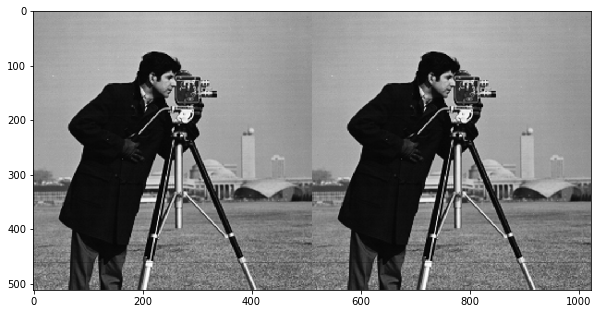
\includegraphics[width=0.7\linewidth]{Machine Learning in Computer Visualisation/img/hstack_image.png}
\end{center}

\subsection{Fading an Image}
\begin{minted}[tabsize=2]{python}
im = skimage.io.imread("data/snoopy.png")
im = im/255 # tip: use floating point values

ims = []

im_temp = np.fliplr(im)
ims.append(im_temp)
for i in range(1,5):
	im_temp = im_temp + (0.4)**i
	ims.append(im_temp)

plt.imshow(np.hstack(ims),vmin=0, vmax=1, cmap="gray")
\end{minted}

\begin{center}
	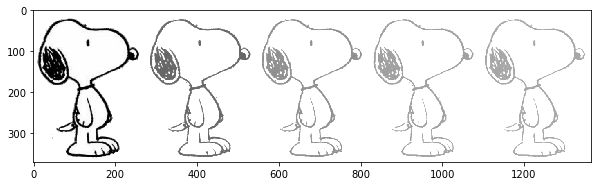
\includegraphics[width=0.7\linewidth]{Machine Learning in Computer Visualisation/img/snoopy_fade.png}
\end{center}

\subsubsection{IPyWidgets}
\begin{minted}[tabsize=2]{python}
@interact(thresh=widgets.FloatSlider(min=0.0, max=0.5, step=0.01, value=0.2))
def threshold(thresh):
	im_thresh = []
	for line in im:
		im_thresh.append([pixel if pixel > np.min(line) 
			+ thresh else float(0) for pixel in line])
	plt.imshow(im_thresh, cmap="gray", vmin=0, vmax=1)
	plt.show()
\end{minted}

\begin{center}
	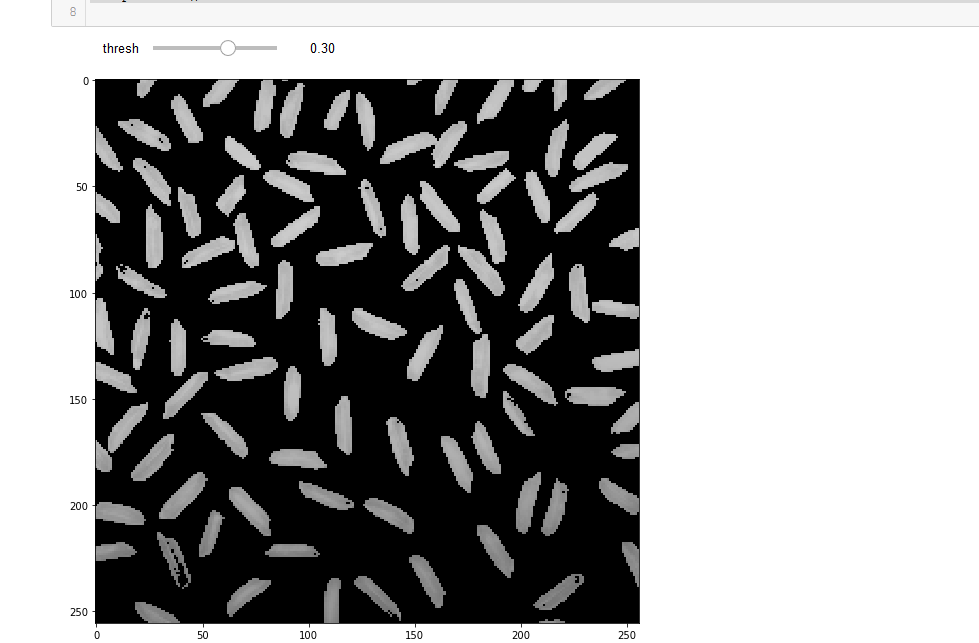
\includegraphics[width=0.6\linewidth]{Machine Learning in Computer Visualisation/img/ipywidgets_example.png}
\end{center}


\section{Local Filtering and Edge Detection}
\subsection{Filtering}
The naive approach of local filtering is taking just a moving average of the pixels in the neighbourhood.

\subsection{Moving average}
\begin{center}
	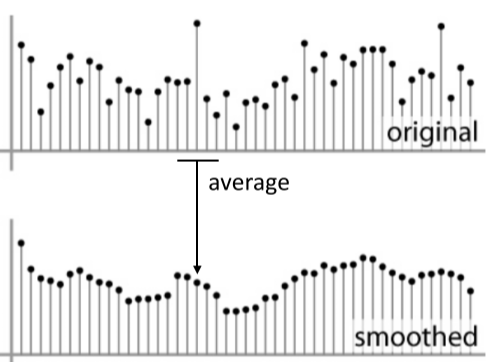
\includegraphics[width=0.6\linewidth]{Machine Learning in Computer Visualisation/img/MovingAverage.PNG}
\end{center}
\begin{equation}
     b_{smoothed}[i] = \frac{1}{2r+1} \sum_{j=i=-r}^{i+r} b[j] 
\end{equation}

 \begin{center}\begin{tabular}{rclcrcl}
   $r$ & = & range of the points  \\ 
   $b$ & = & Point \\
\end{tabular}\end{center}

\subsection{Convolution}
Convolve an input matrix (the input image) with a \textbf{kernel}, which is a matrix defining a weight for every element of the neighbourhood. The convolution can be considered a moving weighted average of the pixels.

\textbf{1D Example}
\begin{equation}
     (a\ast b)[i] = \sum_{j}^{} a[j]b[j-1] 
\end{equation}

 \begin{center}\begin{tabular}{rclcrcl}
   $a$ & = & Filter e.g.  [1,4,6,4,1]/16\\ 
   $b$ & = & Point \\
\end{tabular}\end{center}


\textbf{2D Example}
\begin{equation}
     (a\ast b)[i,j] = \sum_{j',j'}^{} a[i',j']b[i-i',j-j'] 
\end{equation}

 \begin{center}\begin{tabular}{rclcrcl}
   $a$ & = & Filter e.g.  [1,4,6,4,1]/16\\ 
   $b$ & = & Point \\
\end{tabular}\end{center}


\begin{center}
	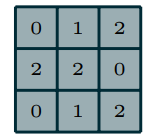
\includegraphics[width=0.4\linewidth]{Machine Learning in Computer Visualisation/img/Kernel_Convolution.png}
\end{center}
This kernel slides across the input matrix. At each location, the product between each element of the kernel and the input element it overlaps is computed and the results are summed up to obtain the output in the current location. In general, if the input matrix has  $i$ rows and the kernel has $k$ rows, the output will have $i-k+1$ rows, the same applies to columns.
\begin{center}
	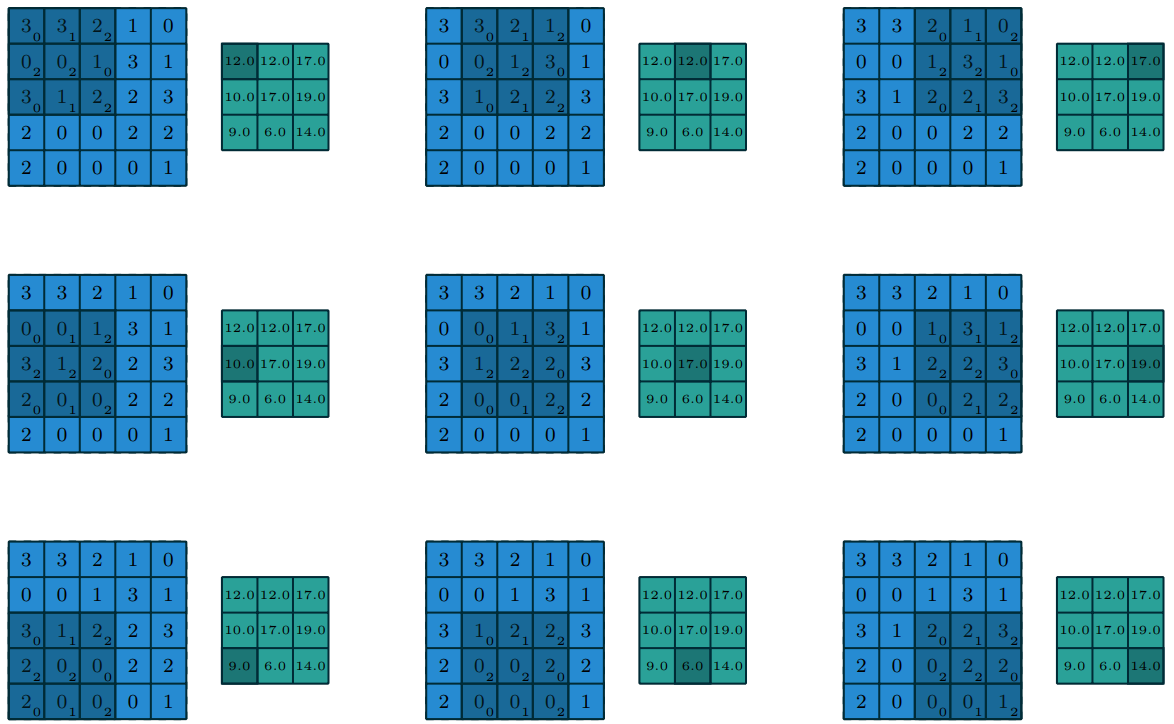
\includegraphics[width=0.8\linewidth]{Machine Learning in Computer Visualisation/img/ConvolutionOutput.png}
\end{center}


\subsubsection{Smooth filter}
This smoothes the picture.
\begin{center}
    $ \frac{1}{9}\begin{bmatrix}
    1 & 1 & 1 \\
    1 & 1 & 1 \\
    1 & 1 & 1 
    \end{bmatrix}  $
\end{center}
Usually done with a Gaussian filter.


\subsubsection{Sharpening filter}
This smoothes the picture.
\begin{equation}
\begin{bmatrix}
    0 & 0 & 0 \\
    0 & 2 & 0 \\
    0 & 0 & 0 
    \end{bmatrix} 
    -
    \frac{1}{9}\begin{bmatrix}
    1 & 1 & 1 \\
    1 & 1 & 1 \\
    1 & 1 & 1 
    \end{bmatrix}
    =
    \frac{1}{9}\begin{bmatrix}
    -1 & -1 & -1 \\
    -1 & 17 & -1 \\
    -1 & -1 & -1 
    \end{bmatrix}
\end{equation}

\begin{center}
	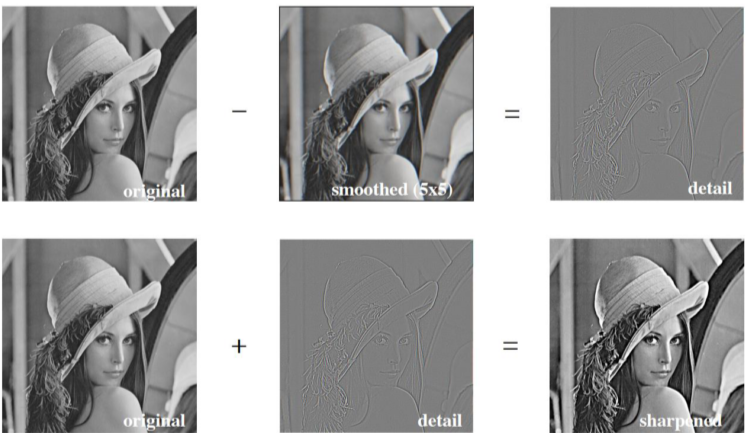
\includegraphics[width=0.6\linewidth]{Machine Learning in Computer Visualisation/img/sharpening.PNG}
\end{center}

\subsection{Gaussian filter}
\begin{center}
	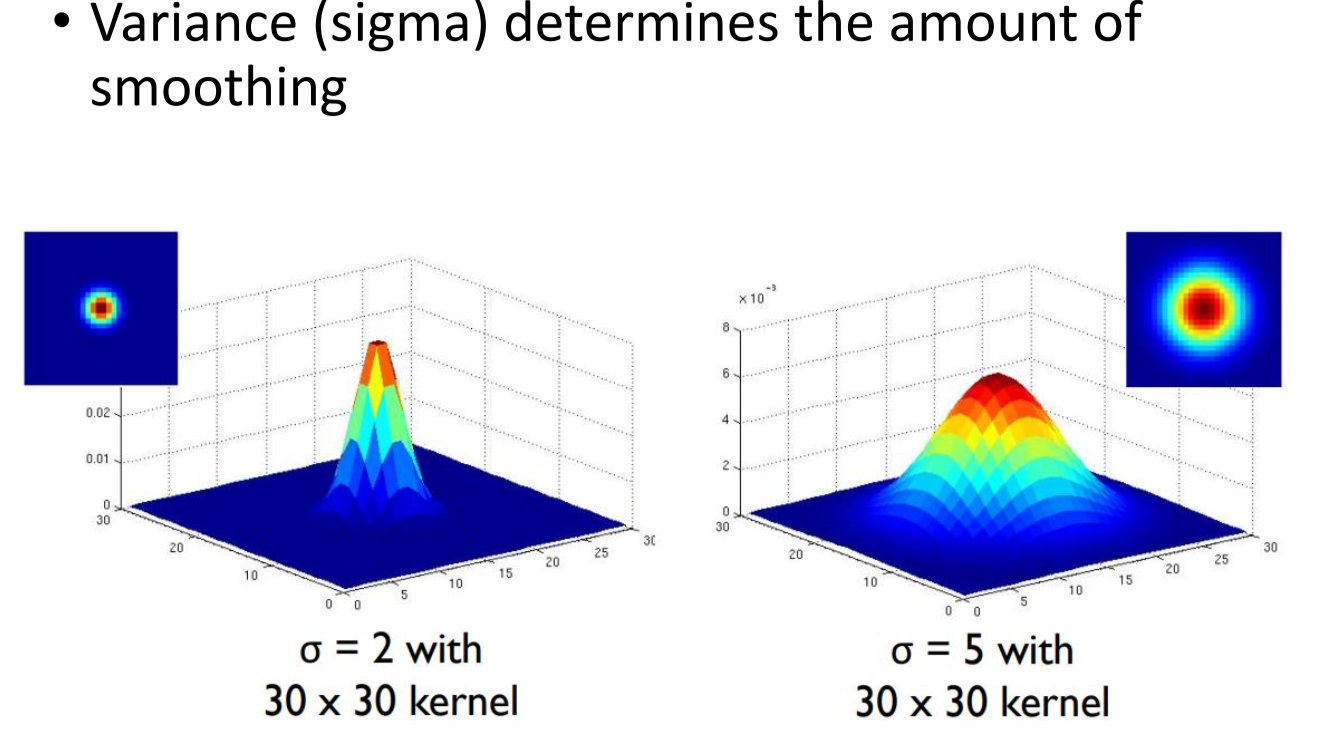
\includegraphics[width=0.8\linewidth]{Machine Learning in Computer Visualisation/img/GaussFilter.PNG}
\end{center}

\noindent A Gaussian filter has a symmetrical value increase from outside to inside, with the highest value in the middle.

\begin{equation}
\frac{1}{16}
\begin{bmatrix}
    1 & 2 & 1 \\
    2 & 4 & 2 \\
    1 & 2 & 1 
    \end{bmatrix} 
\end{equation}

\subsection{Edge Detection}
Although intuitive for humans to detect, edge detection was a hard problem in image processing. And edge is defined by a rapid change in the intensity, which can be exploited by calculating the derivative.

\begin{center}
	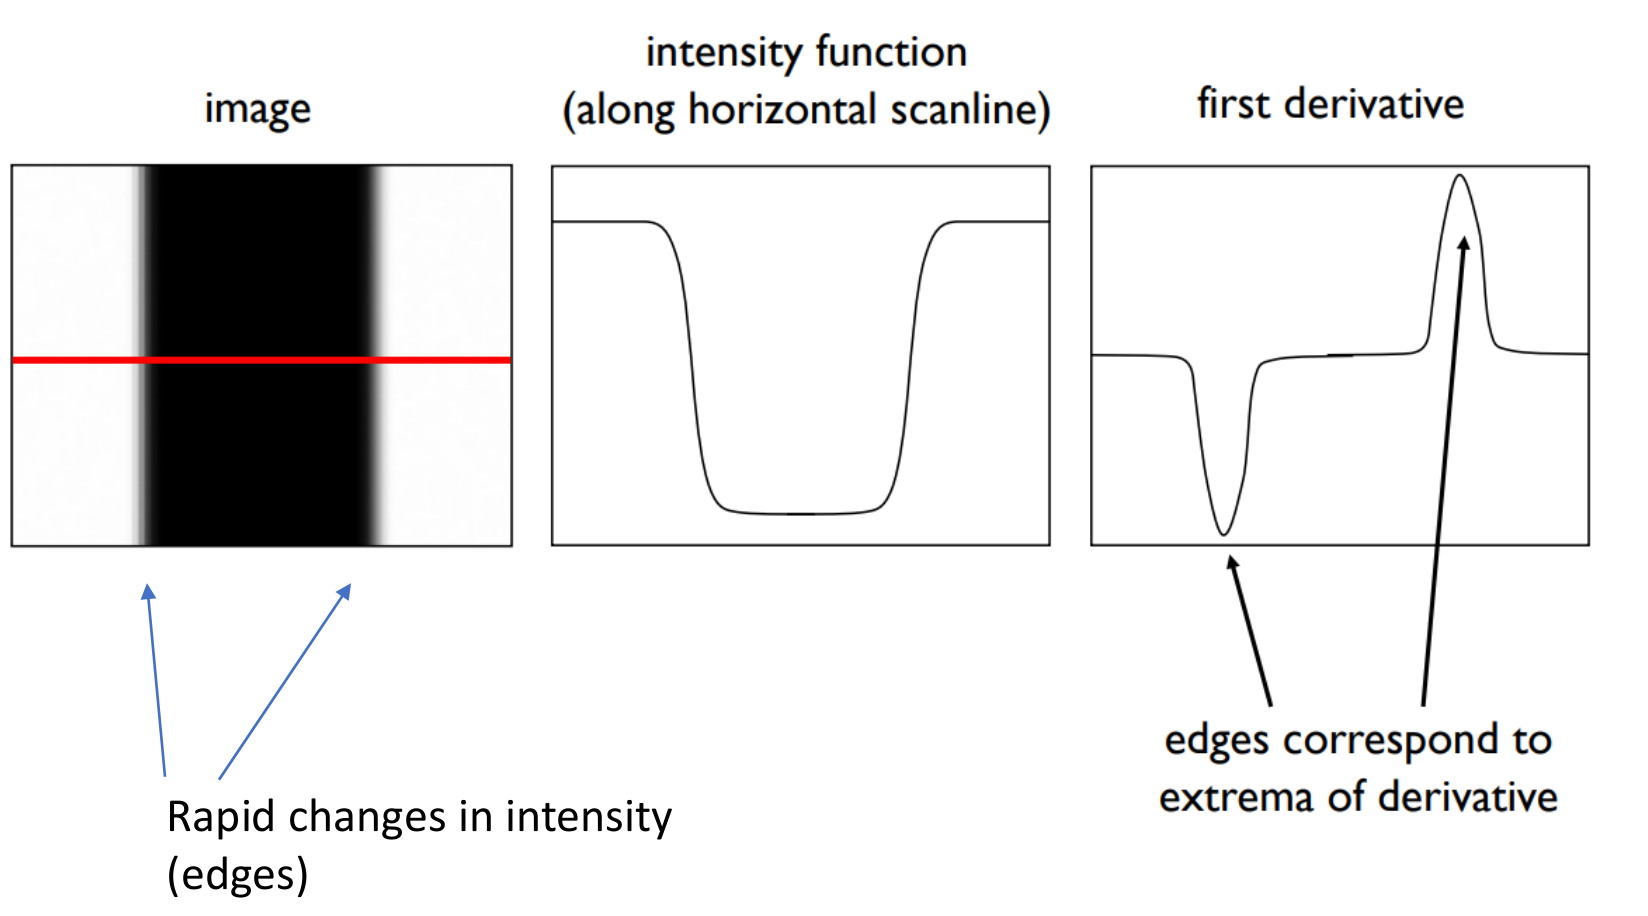
\includegraphics[width=0.6\linewidth]{Machine Learning in Computer Visualisation/img/1D_edge_derivative.png}
\end{center}

\noindent
In two dimensions the derivative corresponds to the gradient $\nabla f = \left[\frac{\partial f}{\partial x},\frac{\partial f}{\partial y}\right]$, which points from the edge towards the increase in intensity or the lighter side.

\begin{align}
\shortintertext{Gradient}
\nabla f &= \left[ \frac{\partial f}{\partial x}, \frac{\partial f}{\partial y} \right]
\shortintertext{Gradient Direction}
\theta &= \tan^{-1} \left( \frac{\partial f}{\partial x} / \frac{\partial f}{\partial y} \right)
\shortintertext{Gradient Magnitude (strength of the edge)}
\norm{\nabla f} &= \sqrt{\left(\frac{\partial f}{\partial x}\right)^2 + \left(\frac{\partial f}{\partial y} \right)^2 }
\end{align}

But not all important edges have strong gradients, nor are all strong gradients important edges.

\begin{figure}[H]
	\centering
	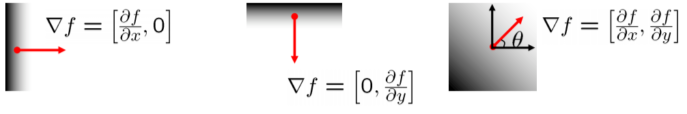
\includegraphics[width=0.6\linewidth]{Machine Learning in Computer Visualisation/img/Gradient.PNG}
	\caption{Gradient goes from black to white}
	\label{fig:Gradient_verlauf}
\end{figure}

\subsubsection{Computing the Gradient on an Image}
Approximate Gradient in direction of $ \frac{\partial f}{\partial x} $: Convolution with kernel \begin{tabular}{|c|c|}
	\hline
	-1 & 1\\
	\hline
\end{tabular}

\noindent
Approximate Gradient in direction of $ \frac{\partial f}{\partial y} $: Convolution with kernel \begin{tabular}{|c|}
	\hline
	-1 \\
	\hline
	1\\
	\hline
\end{tabular}

The drawback of the gradient is, that it is very sensitive to noise:
\begin{figure}[H]
	\centering
	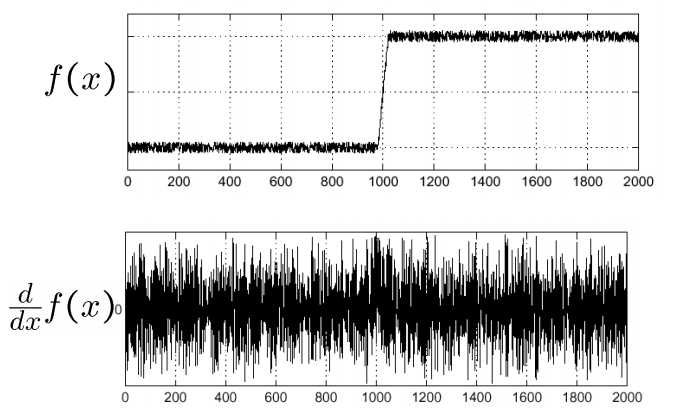
\includegraphics[width=0.7\linewidth]{Machine Learning in Computer Visualisation/img/noise_gradient.png}
	\caption{Gradient of a 1D function, where it is clear how it amplifies noise and may conceal a weak signal}
	\label{fig:noisegradient}
\end{figure}

\noindent
The solution to this is, to first smooth the function and then apply the gradient.

The larger the value of $\sigma$ the more smoothing is applied and different kind of features can be identified.
\begin{itemize}[leftmargin=*, labelindent=3.5cm, labelsep=0.5cm]
	\item[\textbf{large value of $\sigma$}] larger scale or stronger edges detected
	\item[\textbf{smaller value of $\sigma$}] finer details detected
\end{itemize}

\begin{figure}[H]
	\centering
	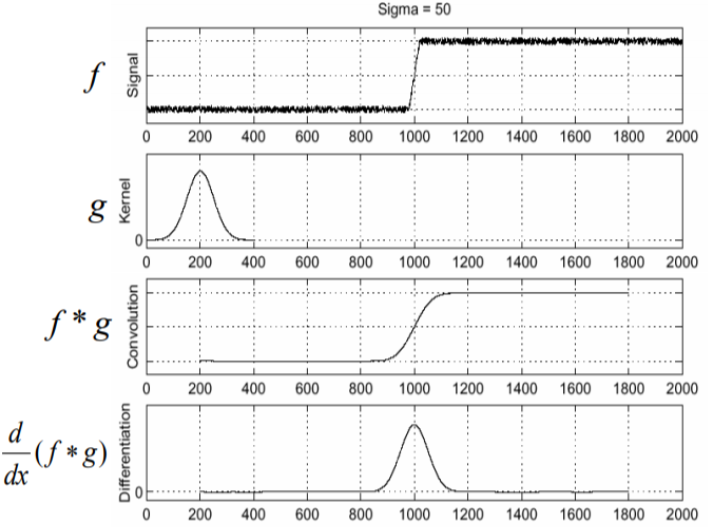
\includegraphics[width=0.6\linewidth]{Machine Learning in Computer Visualisation/img/Gradient_withGauss.PNG}
	\caption{Gradient with Gaussian smoothing}
	\label{fig:noisegradient-smoothed}
\end{figure}


\noindent
\begin{minipage}{0.6\textwidth}
	In practice a convolution with a derivative of Gaussian filter is calculated to compute the gradients.
	
	This is equivalent to smoothing with a Gaussian and then taking the derivative.
\end{minipage}
\begin{minipage}{0.4\textwidth}
	\begin{center}
		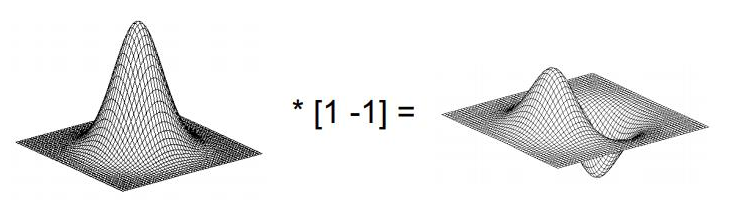
\includegraphics[width=0.6\linewidth]{Machine Learning in Computer Visualisation/img/derivative_gaussian_filter.png}
	\end{center}
\end{minipage}

\begin{figure}[H]
	\centering
	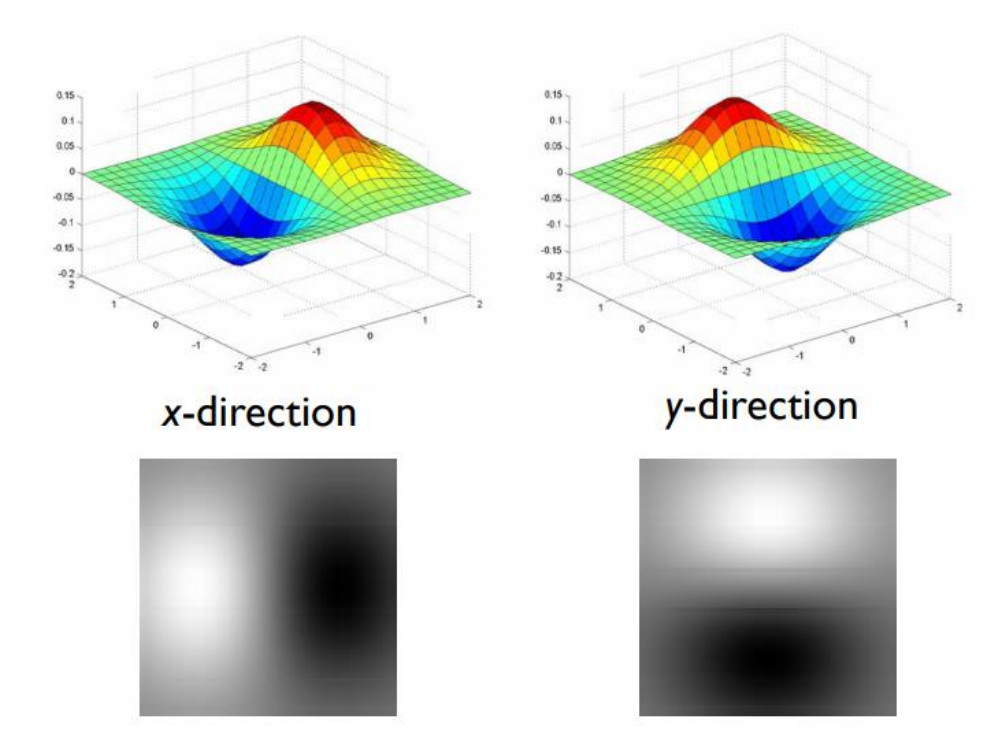
\includegraphics[width=0.6\linewidth]{Machine Learning in Computer Visualisation/img/derivative_gaussian_filter2.png}
	\caption{Derivative of Gaussian Filters}
	\label{fig:derivativegaussianfilter2}
\end{figure}

\begin{itemize}
	\item A Gaussian smoothing filter removes high-frequency components
	\item Values of a Gaussian smoothing filter sum to one
	\item Derivative filters contain some negative value and values sum to zero
	\item Derivative filters yield large responses at points with high contrast
\end{itemize}


\subsection{Canny Edge Detection}
Same base approach but enhanced with edge thinning and hysteresis thresholding.\footnote{A good explanation with sample code can be found under \href{https://docs.opencv.org/4.3.0/da/d22/tutorial_py_canny.html}{OpenCV Canny Edge Detection Tutorial}}
\newline
\textbf{Canny Edge Algorithm}
\begin{enumerate}
	\item Approximate gradients along axes by derivative of Gaussian filters
	\item Compute gradient magnitude
	\item Make edge one pixel wide, thinning through \textbf{non-maxima suppression} along perpendicular direction to the edge
	\item Only keep strong edges through hysteresis thresholding 
\end{enumerate}

\subsubsection{Non-maxima suppression}
Only keep the maxima of a line
\begin{figure}[H]
	\centering
	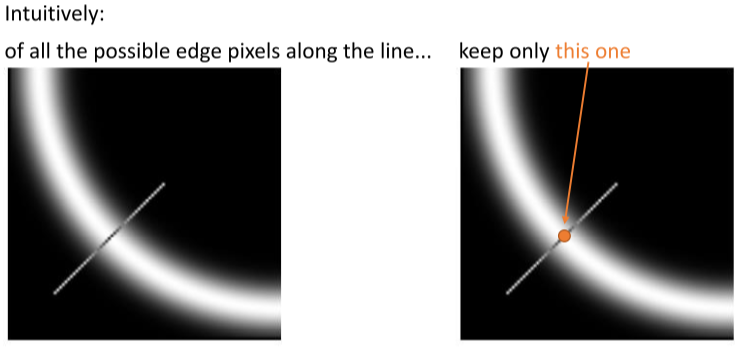
\includegraphics[keepaspectratio,width=0.6\linewidth]{Machine Learning in Computer Visualisation/img/NonMaimaSupression.PNG}
	\caption{Non-maxima impression. Results in thinning the edge to a 1 Pixel width.}
\end{figure}

\subsubsection{Hysteresis Thresholding}
This stage decides which are all edges are really edges and which are not. For this, two threshold values, minVal and maxVal, are needed. Any edges with intensity gradient more than maxVal are sure to be edges and those below minVal are sure to be non-edges, and are thus discarded. Those who lie between these two thresholds are classified edges or non-edges based on their connectivity. If they are connected to "sure-edge" pixels, they are considered to be part of edges. Otherwise, they are also discarded.
	
\begin{figure}[H]
	\centering
	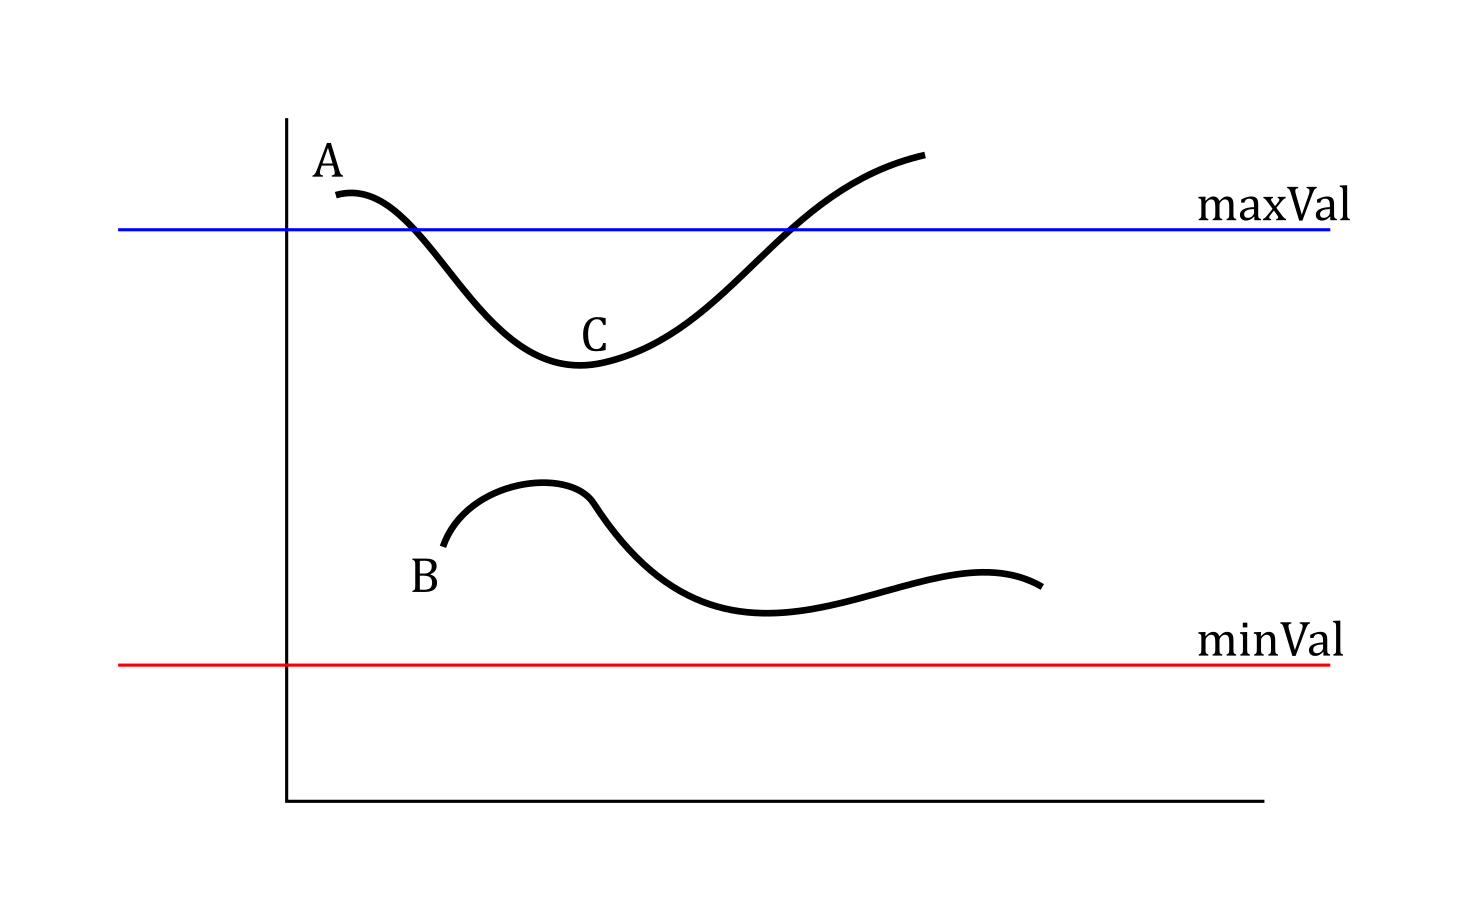
\includegraphics[keepaspectratio,width=1\linewidth]{Machine Learning in Computer Visualisation/img/hysteresis_thresholding.png}
	\caption{Hysteresis thresholding for edge detection. Edges lower than the high threshold are only looked at if before were higher than the high threshold}
\end{figure}

\section{Model Fitting and Line and Circle Detection}
Edge detection is usually not enough as there are usually more than one line in an image and many edges that do not belong to a line. There might be noise in the edges belonging to a line which brings them out of alignment. Lines might also not be complete.

\subsection{Model Fitting}
Model fitting is an algorithm that finds or fits a high-level explanation or model that explains the observations well. In this case the edges are the observations and the model are one or more line.

\subsection{Voting Algorithms}
Voting algorithms are a general technique for decision methods.

\begin{enumerate}
	\item \textbf{Every feature casts votes for all models that are compatible with it}
	\item \textbf{Choose models that accumulate a lot of votes}
\end{enumerate}

Clutter and noise will cast a lot of votes, but are inconsistent. Instead, features belonging to a model will concentrate a lot of votes for that model.

\subsection{Hough Transform}
\begin{enumerate}
	\item Every \textbf{edge point} casts votes for \textbf{all lines that are compatible} with it
	\item Choose \textbf{lines} that accumulated a lot of votes
\end{enumerate}

\textbf{Hough line to point}
\begin{equation}
    y = m_0x+b_0
\end{equation}

\begin{figure}[H]
	\centering
	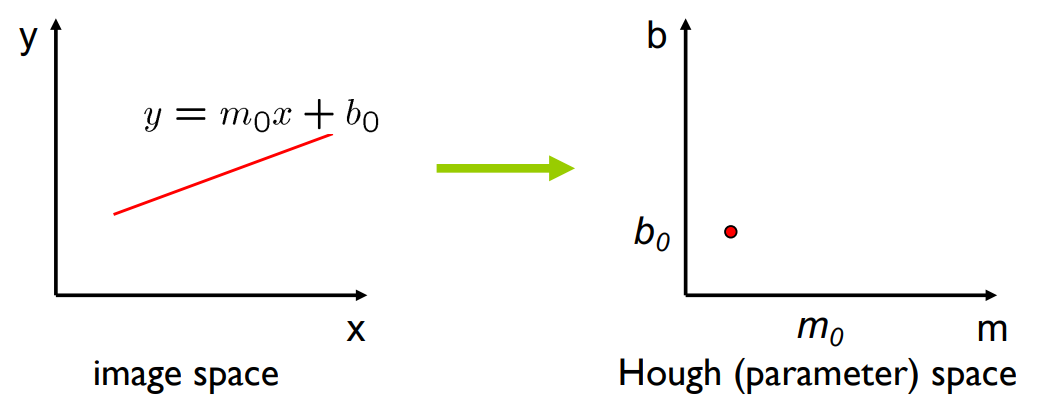
\includegraphics[width=0.8\linewidth,keepaspectratio]{Machine Learning in Computer Visualisation/img/line_representation_hough.png}
	\caption{Line representation in Hough space}
\end{figure}

\textbf{Hough line to point}
\begin{equation}
    b = -xm_0+y_0
\end{equation}
This means drawing a line for every $m_0$. (To draw, set two $m_0$ and draw the line and extend it...)

\begin{figure}[H]
	\centering
	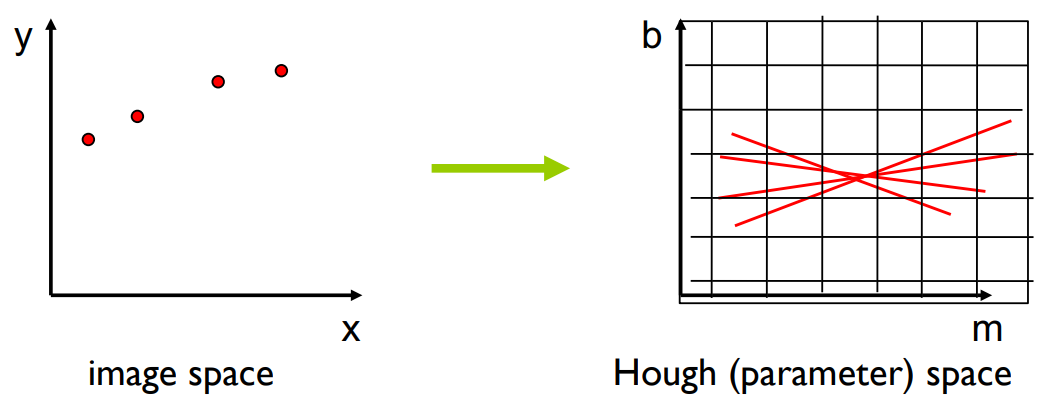
\includegraphics[width=0.8\linewidth]{Machine Learning in Computer Visualisation/img/points_representation_hough.png}
	\caption{Points on a line in normal space almost intersect in Hough space}
	\label{fig:pointsrepresentationhough}
\end{figure}

\begin{figure}[H]
	\centering
	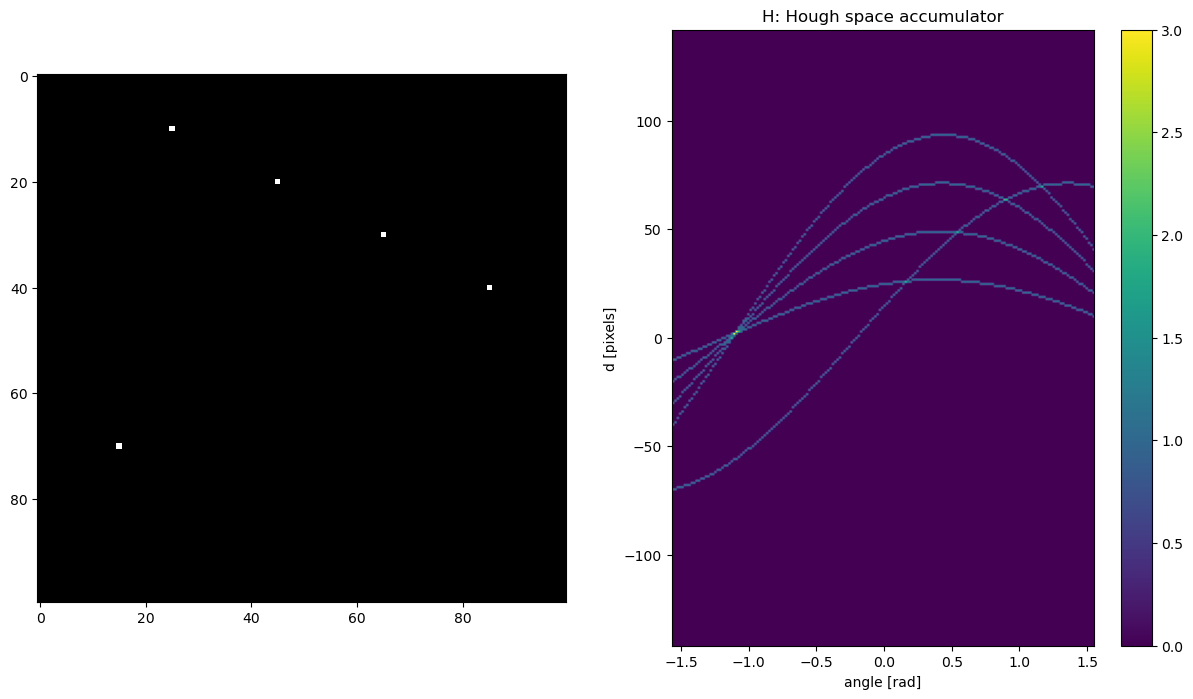
\includegraphics[width=0.7\linewidth]{Machine Learning in Computer Visualisation/img/hough_uebungen.png}
	\caption{Points on a line intersect in Hough space}
	\label{fig:pointsrepresentationhough}
\end{figure}



\noindent
The problem with this approach is that
\begin{enumerate}[label=\alph*.]
	\item the parameter space $(m,b)$ is \textbf{not bounded}
	\item \textbf{vertical lines} can not be represented
\end{enumerate}

\subsection{Representation of Lines in Polar Coordinates}

The angle 0 is located on the x-axis to the right $\rightarrow$.

\begin{equation}
     \theta = \{0^\circ,360^\circ \}
     d = \{ 0^\circ, \sqrt{x_{max}^2 + y_{max}^2} \}
\end{equation}

\begin{equation}
     d = \{ 0^\circ, \sqrt{x_{max}^2 + y_{max}^2} \}
\end{equation}

 \begin{center}\begin{tabular}{rclcrcl}
   $\theta$ & = & Angle in degree\\ 
   $d$ & = & distance from line to origin \\
\end{tabular}\end{center}

\begin{figure}[H]
	\centering
	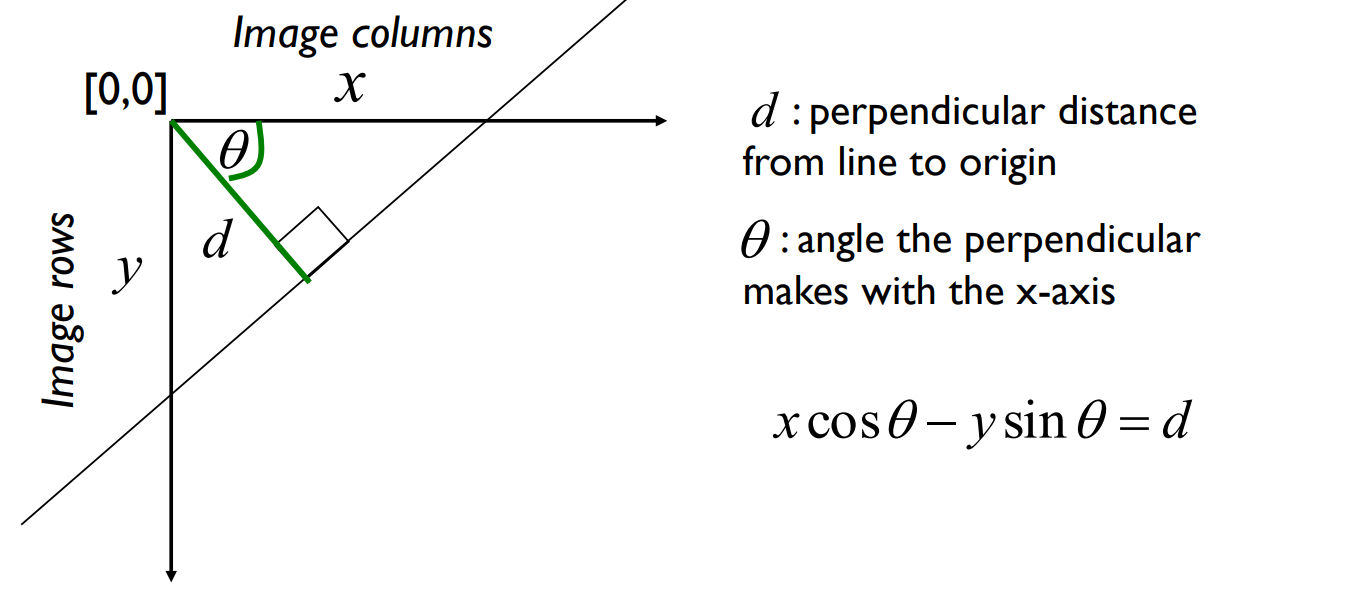
\includegraphics[width=0.8\linewidth]{Machine Learning in Computer Visualisation/img/line_representation_polar.png}
	\caption{Line representation with polar parameters}
	\label{fig:linerepresentationpolar}
\end{figure}

\noindent This approach solves both the problem of unboundedness and representation. The parameter $\theta$ is bounded by $[0,2\pi]$ and $d$ by $[0,\text{imagewidth}]$.

\noindent For every point in normal space there will be a Sinusoid the polar Hough space.

\subsection{Hough Transformation Algorithm}
The algorithm transforms each edge point in the image to the Hough space, where an Accumulator array gets filled with votes. The bin size of the accumulator is an important hyperparameter, if the size is too small, there will be many weak peaks due to noise, if too large accuracy of locating a line drops, and many votes from clutter might end up in the same bin. A solution is to keep the bin size small but also count votes from neighbors.

\begin{figure}[H]
	\centering
	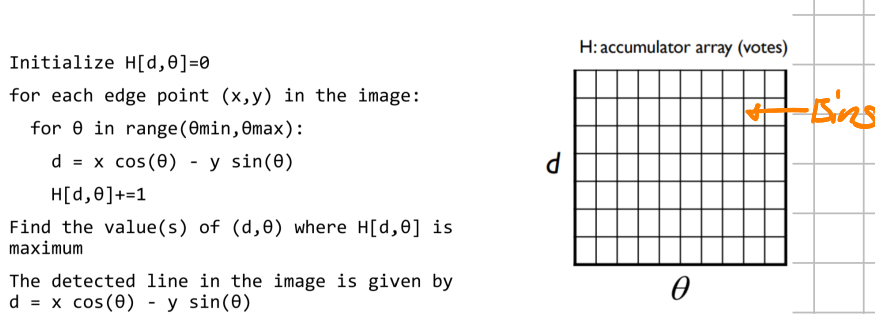
\includegraphics[width=0.8\linewidth]{Machine Learning in Computer Visualisation/img/Hough_ALG.PNG}
	\caption{Hough Algorithm}
	\label{fig:linerepresentationpolar}
\end{figure}
\textbf{Binsize}
\begin{enumerate}
    \item \textbf{Too small:} many weak peaks (Noise)
    \item \textbf{Just right:} one strong peak per line, despite noise
    \item \textbf{Too large:} poor accuracy
\end{enumerate}

\textbf{Solution:} Keep bin size small, also vote for neighbors in the accumulator (Same as smoothing)

\subsubsection{Voting Algorithm for Finding Lines}
\begin{enumerate}
	\item Every edge point casts votes for all lines that are compatible with it
	\item We choose lines that accumulated a lot of votes
\end{enumerate}


\subsubsection{Voting Algorithm for Finding circles}
\begin{enumerate}
	\item Every edge point casts votes for all circles that are compatible with it
	\item We choose circles that accumulated a lot of votes
\end{enumerate}
\begin{theorem}
	Parametrization of a circle
	\begin{equation*}
		(x_i - a)^2 + (y_i - b)^2 = r^2
	\end{equation*}
	With centre $(a,b)$ and radius $r$
\end{theorem}

\begin{center}
	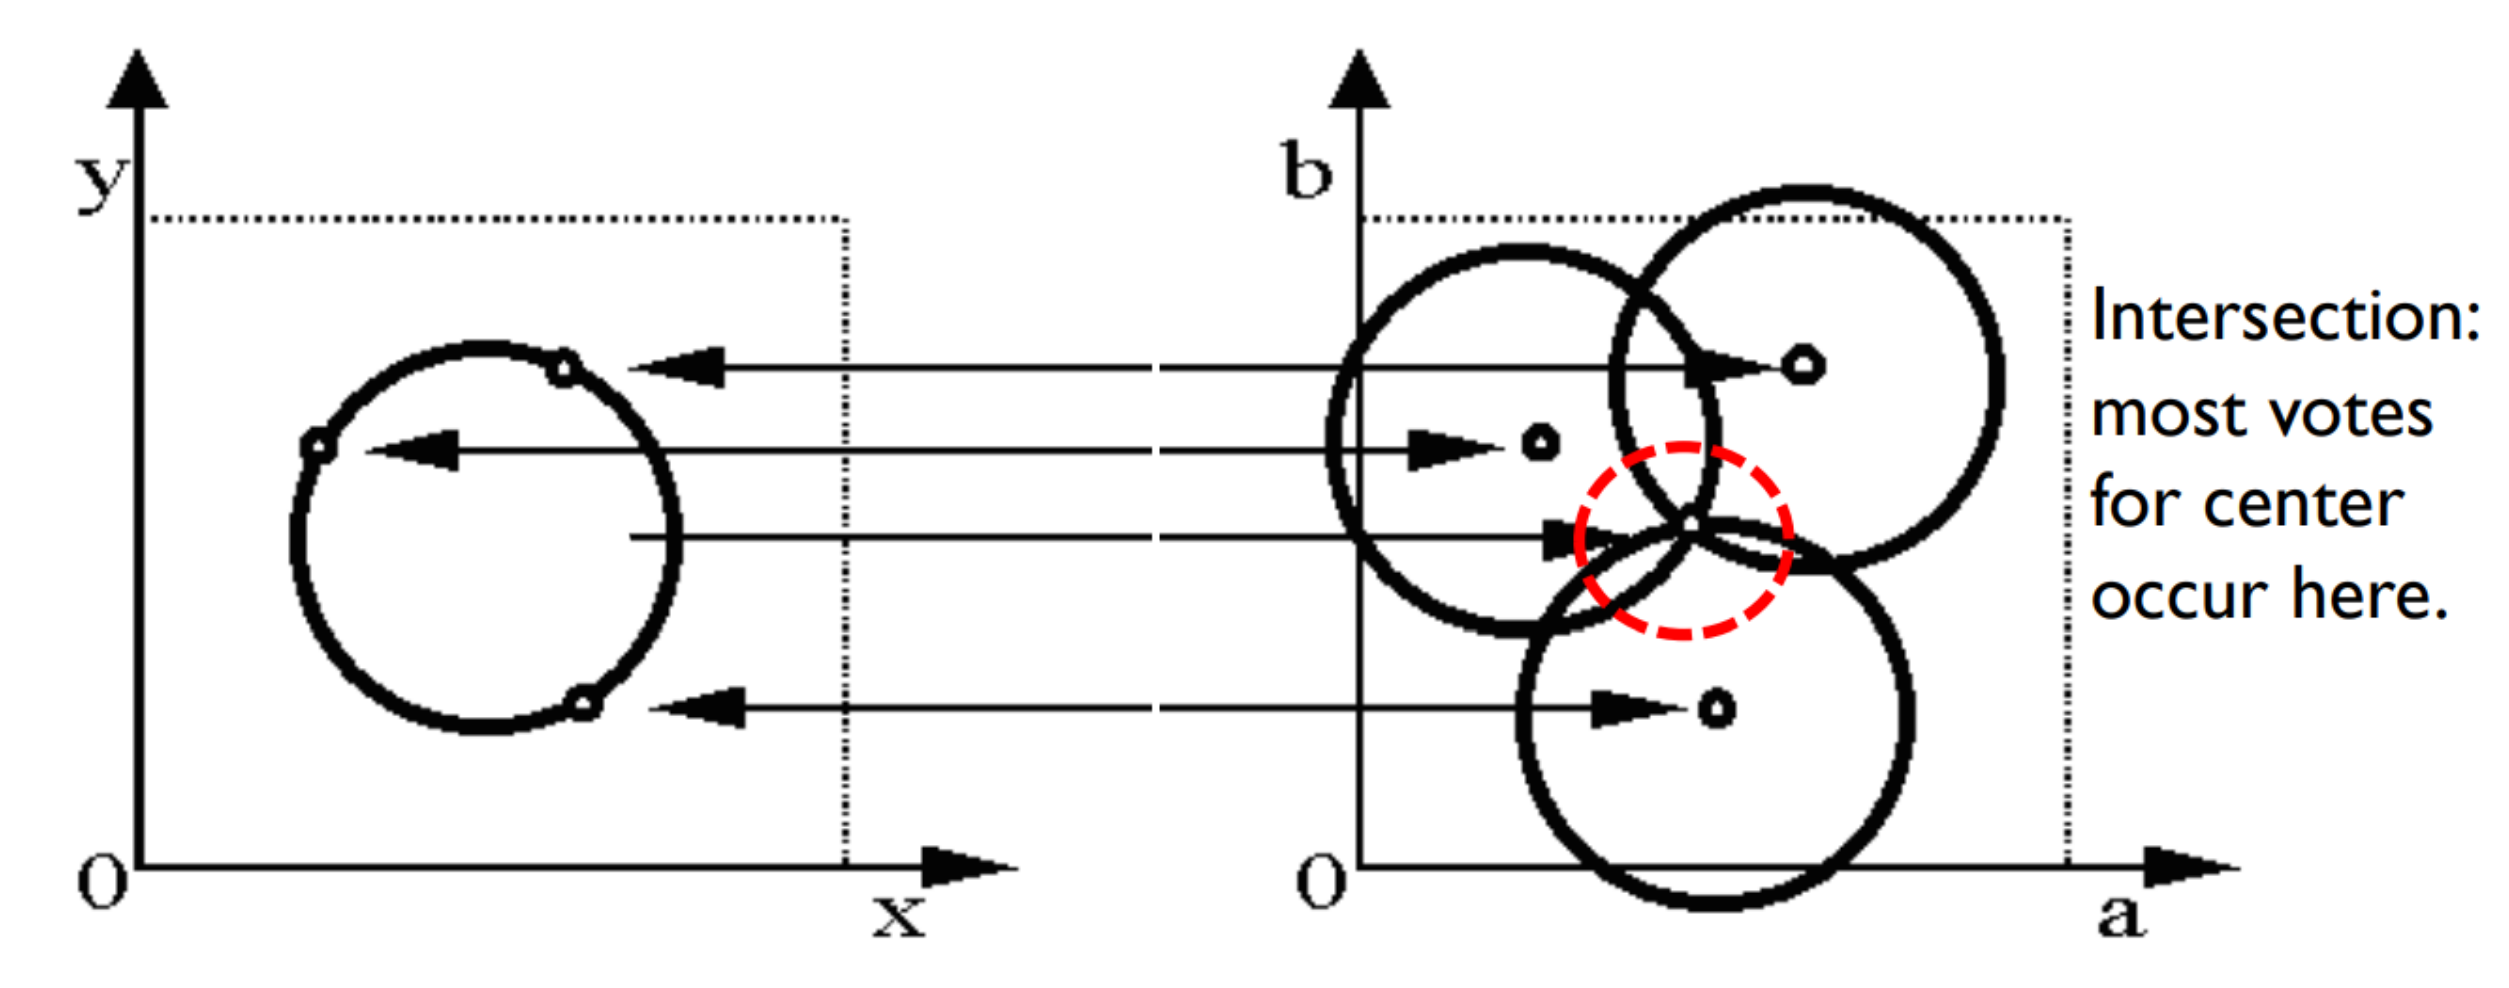
\includegraphics[width=0.7\linewidth]{Machine Learning in Computer Visualisation/img/hough_circle_accumulator.png}
\end{center}

\subsection{Hough Space for Circles With Unknown Radius}

\begin{center}
	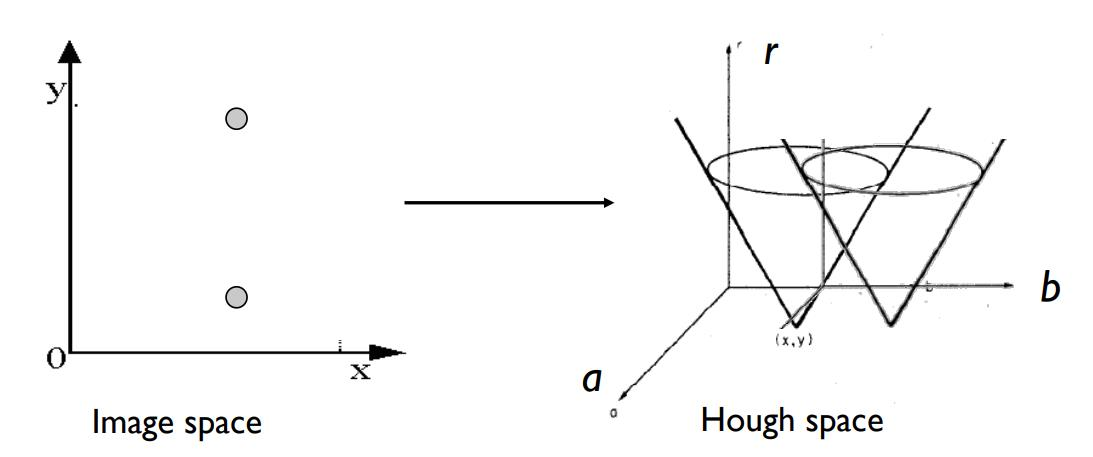
\includegraphics[width=0.7\linewidth]{Machine Learning in Computer Visualisation/img/hough_circle_accumulator_point.png}
\end{center}

\begin{equation*}
	y = a\cdot x + \sout{b}
\end{equation*}


\textbf{Algorithm}
\begin{center}
	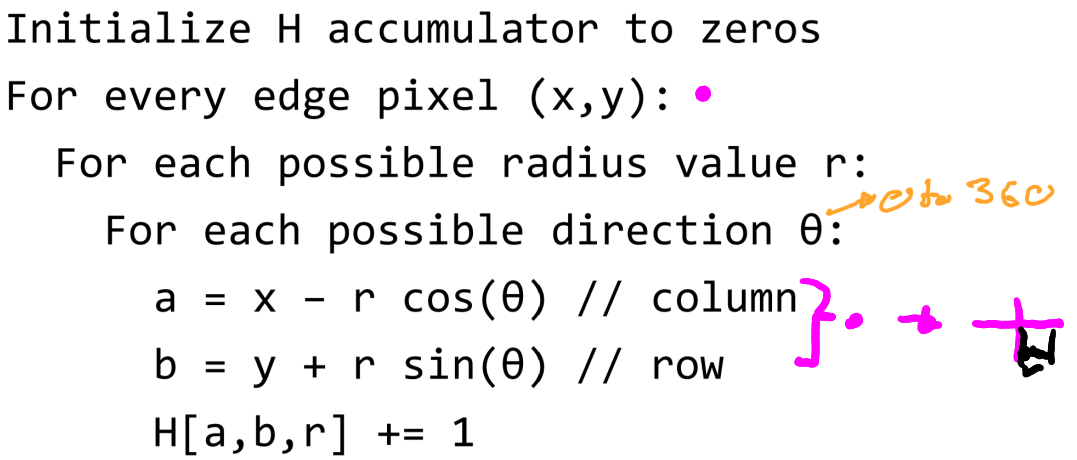
\includegraphics[width=0.7\linewidth]{Machine Learning in Computer Visualisation/img/Circle_Hough.PNG}
\end{center}

\subsection{Hough Space for ellipses}
5 independent parameters define an ellipse. $\rightarrow$ So though space is also 5-dimensional
\begin{center}
	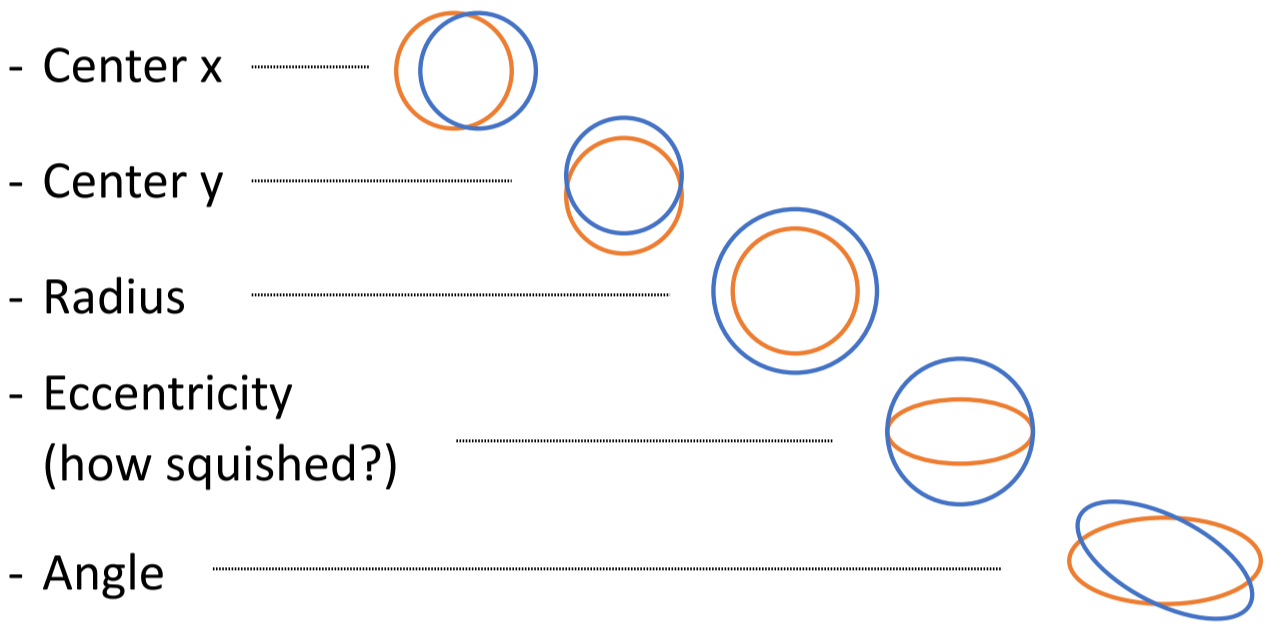
\includegraphics[width=0.7\linewidth]{Machine Learning in Computer Visualisation/img/Hough_Ellipse.PNG}
\end{center}

\section{Image Classification}
Features need a defined database.
\begin{center}
	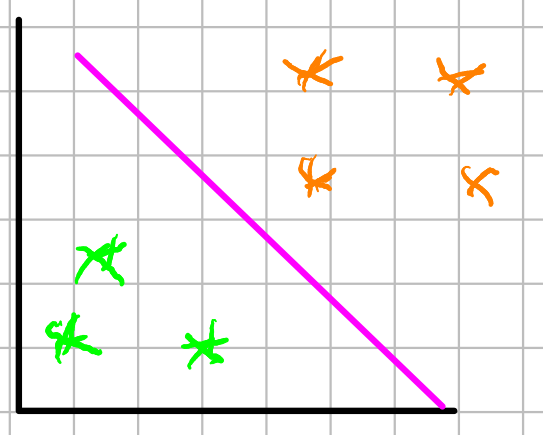
\includegraphics[width=0.4\linewidth]{Machine Learning in Computer Visualisation/img/Aufteilung.PNG}
\end{center}

\subsection{Confusion matrix}
The confusion matrix gives an overview of how the classifier classified.
\begin{equation}
    Accuracy = \frac{Number of correct classifications}{Number of instances in our database}
\end{equation}
\begin{center}
	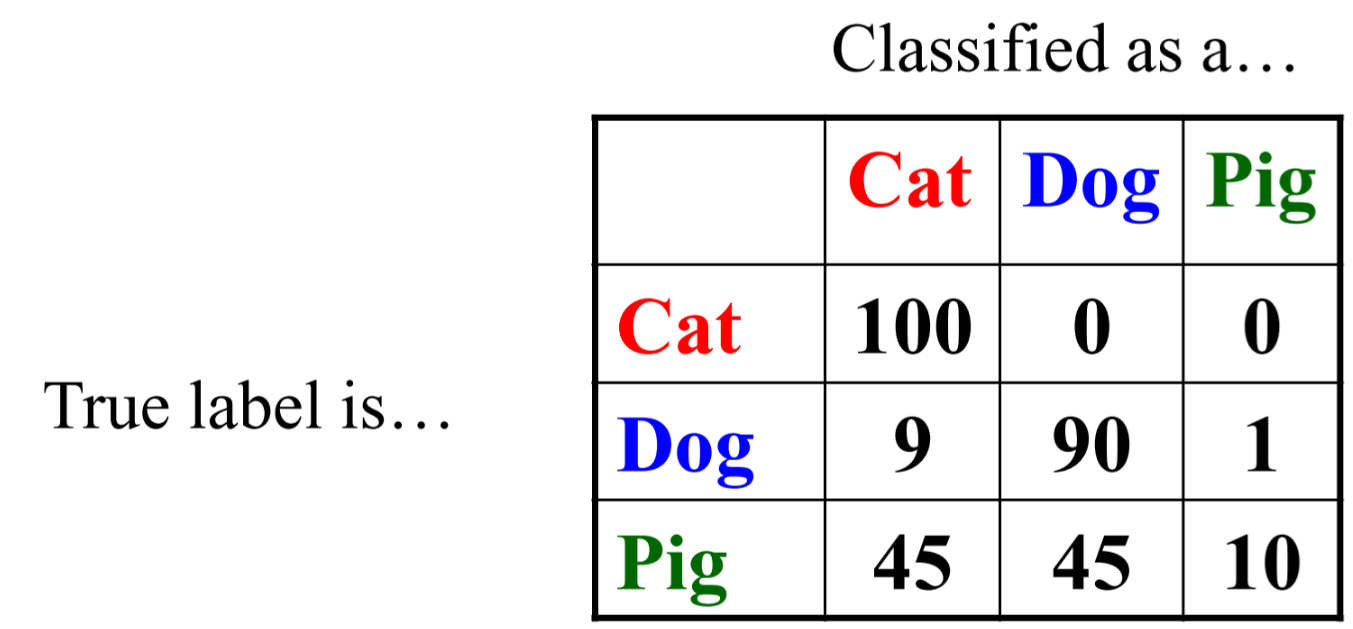
\includegraphics[width=0.5\linewidth]{Machine Learning in Computer Visualisation/img/ConfussionMatrix.PNG}
\end{center}


\subsection{Nearest neighbors}
If the nearest instance of the undeclared instance is an object A then it is an object of type A otherwise it's an object B.
\begin{figure}[H]
     \centering
     \begin{subfigure}[b]{0.45\textwidth}
         \centering
         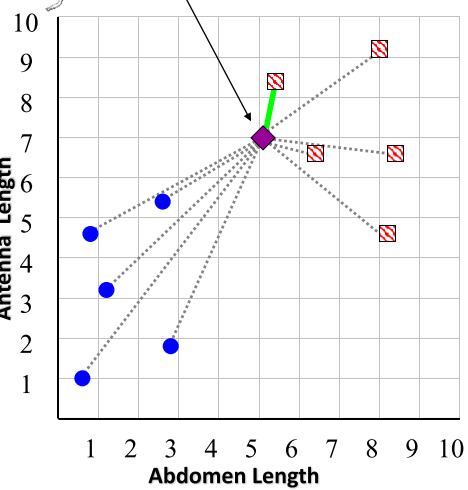
\includegraphics[width=0.95\textwidth]{Machine Learning in Computer Visualisation/img/NearestNeighbour.PNG}
         \caption{Classification  with Nearest neighbor}
     \end{subfigure}
     \hfill
     \begin{subfigure}[b]{0.45\textwidth}
         \centering
         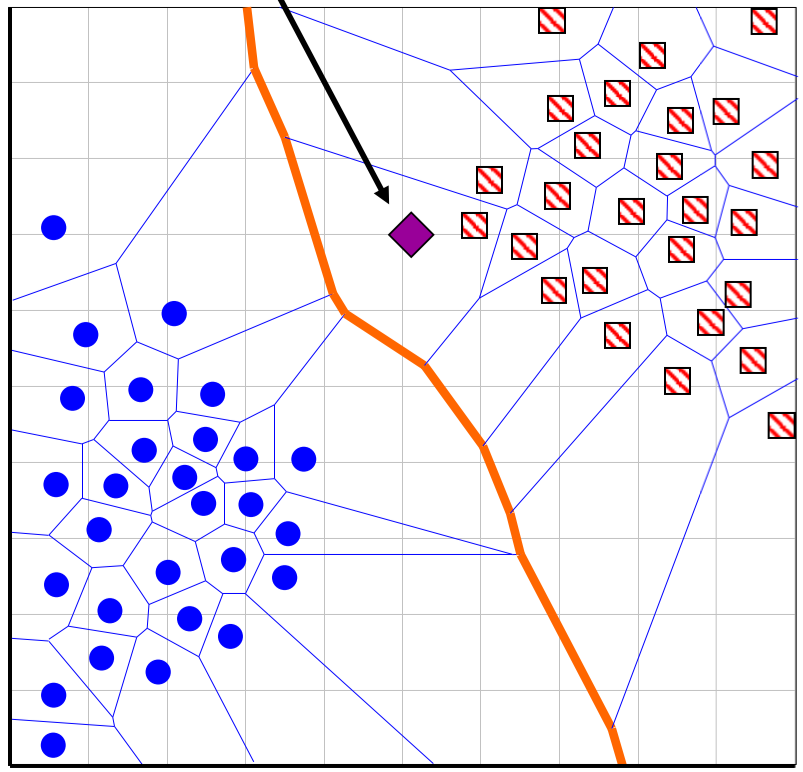
\includegraphics[width=1\textwidth]{Machine Learning in Computer Visualisation/img/Voroni.PNG}
         \caption{Voroni diagram or Theissen regions}
     \end{subfigure}

        \caption{Nearest Neighbors.}
        \label{fig:Start variants}
\end{figure}

\subsection{Training}
\begin{center}
	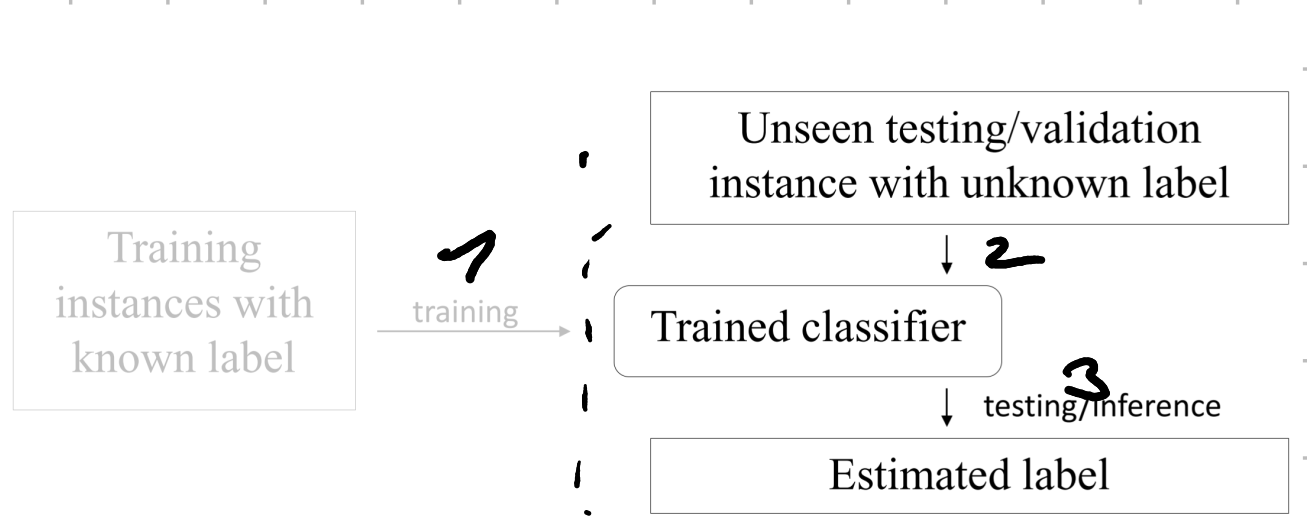
\includegraphics[width=0.7\linewidth]{Machine Learning in Computer Visualisation/img/Training_class.PNG}
\end{center}

\subsection{Convolution neural network}
\begin{center}
	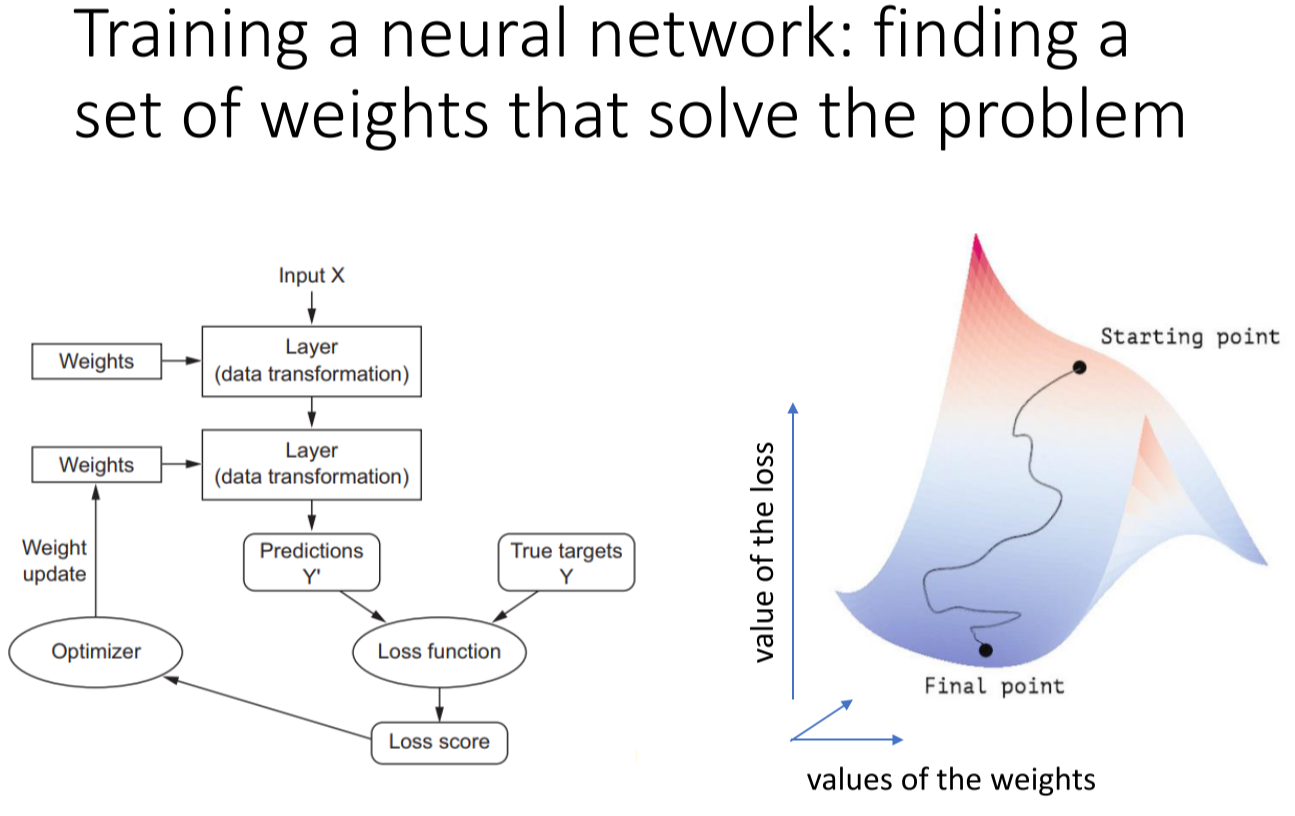
\includegraphics[width=0.7\linewidth]{Machine Learning in Computer Visualisation/img/neuralTraining.PNG}
\end{center}
Number of \textbf{Parameter}
\begin{center}
	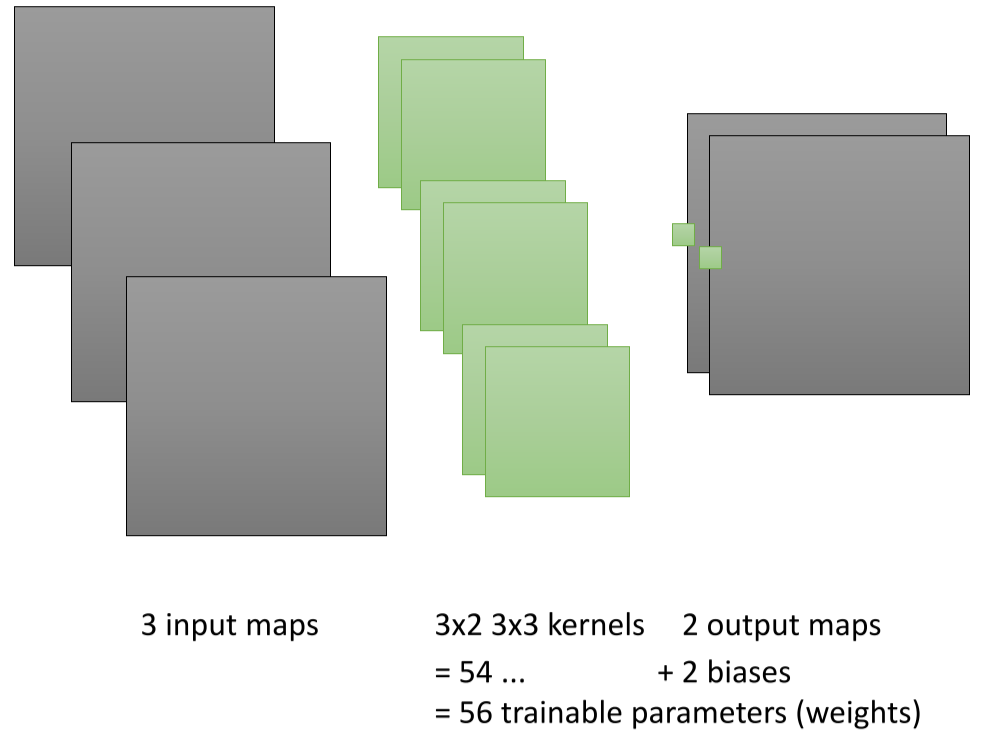
\includegraphics[width=0.7\linewidth]{Machine Learning in Computer Visualisation/img/Parameter.PNG}
\end{center}

\subsubsection{Padding}
How many $n \times n$ patches are fully contained in a $m \times m$ map?
\begin{equation}
    \#fully contained = (m-n+1)\cdot(m-n+1)
\end{equation}
If it should keep the same size, add Padding at the edges to make the $m \times m$ bigger.

\subsubsection{Striding}
Striding means skipping so you can downsample a picture. (The kernel in the picture is 3 x 3)
\begin{center}
	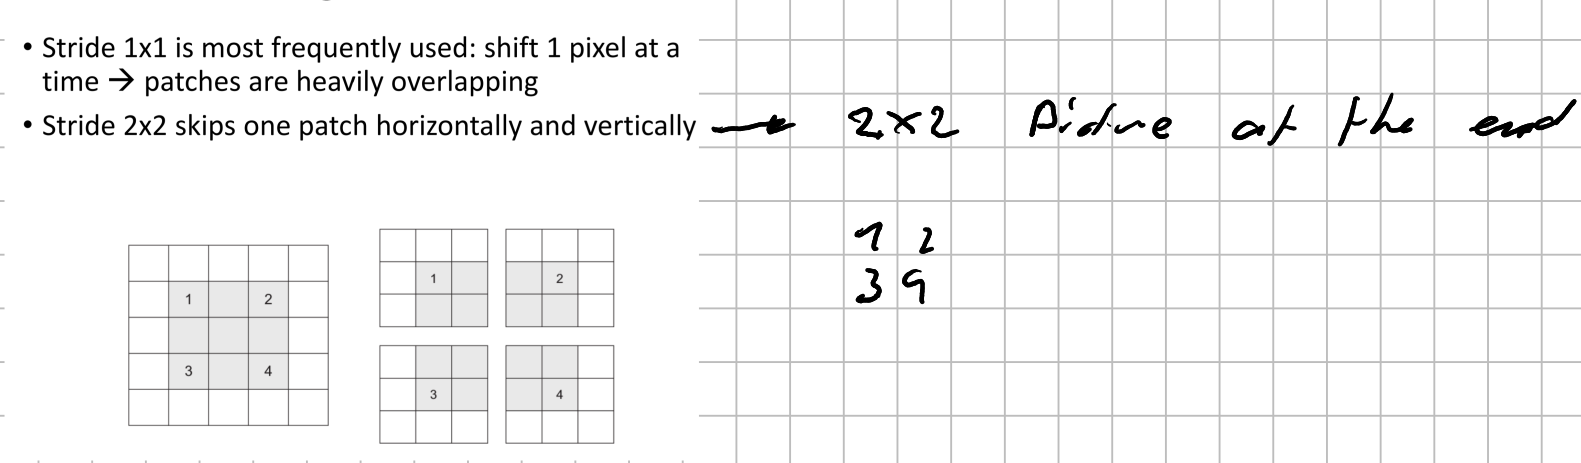
\includegraphics[width=1\linewidth]{Machine Learning in Computer Visualisation/img/Striding.PNG}
\end{center}

\subsubsection{Sparse connectivity and Receptive fields}
\begin{figure}[H]
     \centering
     \begin{subfigure}[b]{0.45\textwidth}
         \centering
         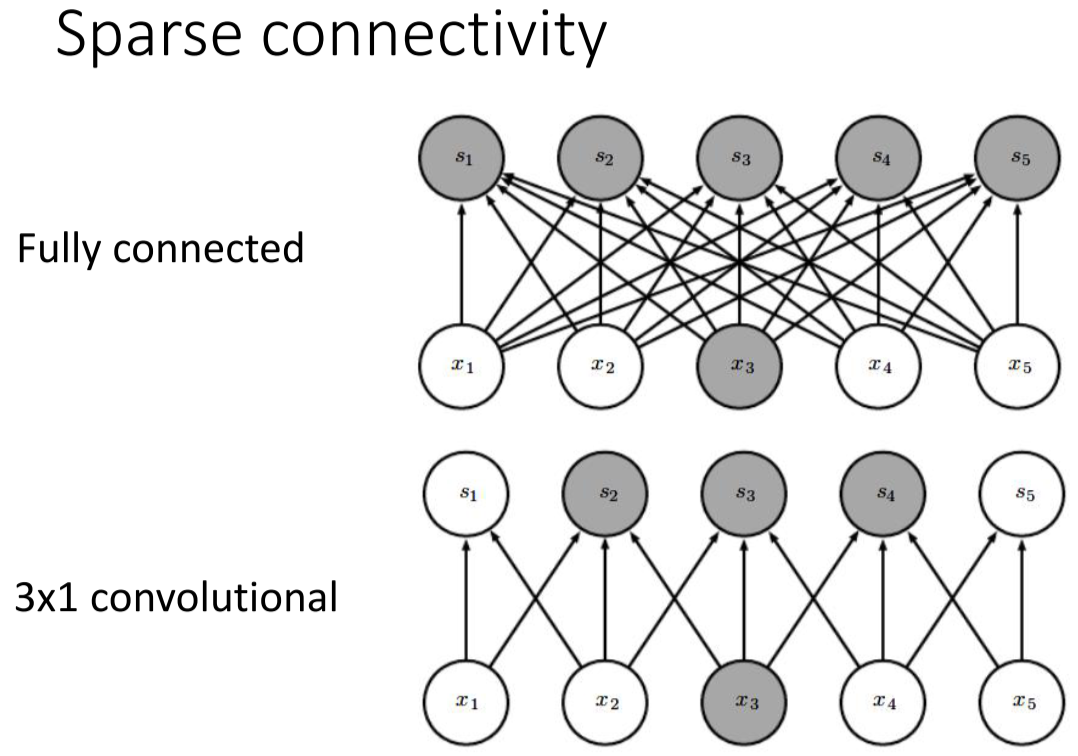
\includegraphics[width=0.95\textwidth]{Machine Learning in Computer Visualisation/img/Sparse.PNG}
         \caption{Sparse connectivity}
     \end{subfigure}
     \hfill
     \begin{subfigure}[b]{0.45\textwidth}
         \centering
         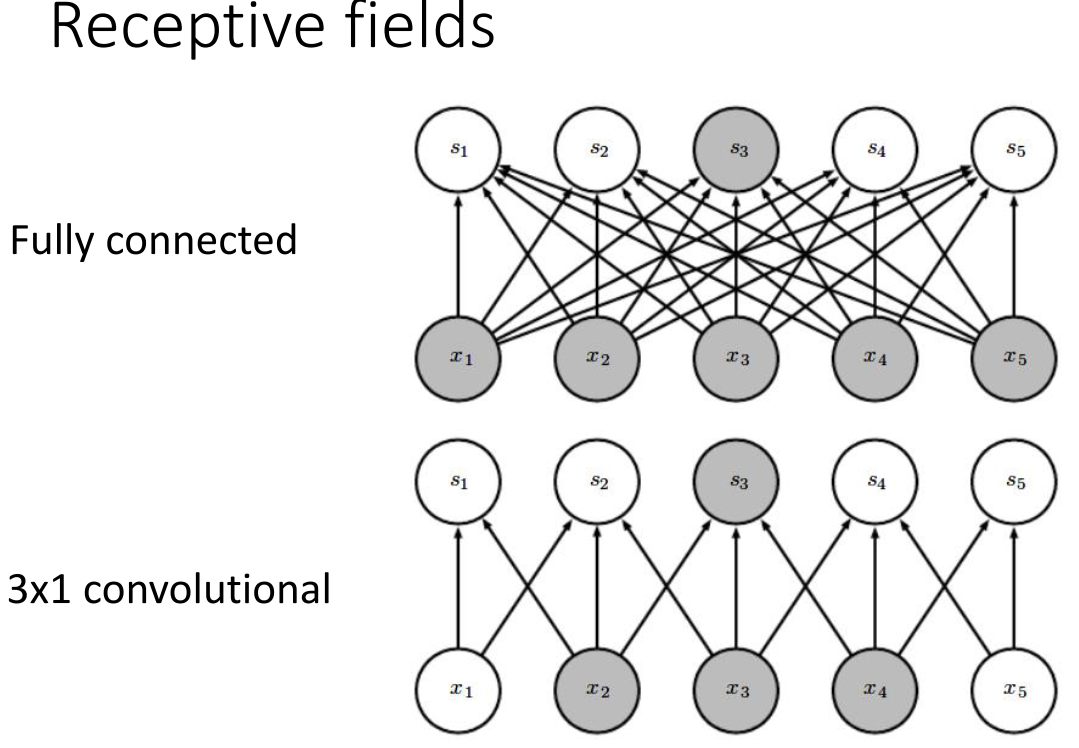
\includegraphics[width=1\textwidth]{Machine Learning in Computer Visualisation/img/receprive.PNG}
         \caption{Receptive fields}
     \end{subfigure}
\end{figure}

\subsubsection{Max pooling}
\begin{figure}[H]
     \centering
     \begin{subfigure}[b]{0.45\textwidth}
         \centering
         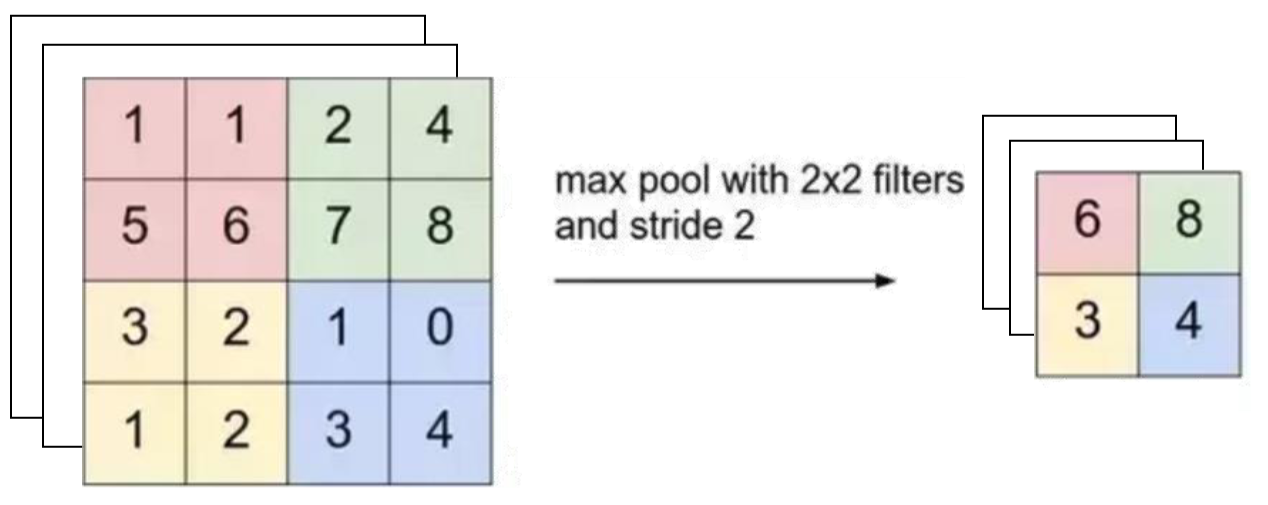
\includegraphics[width=0.95\textwidth]{Machine Learning in Computer Visualisation/img/MaxPooling.PNG}
         \caption{Max pooling}
     \end{subfigure}
     \hfill
     \begin{subfigure}[b]{0.45\textwidth}
         \centering
         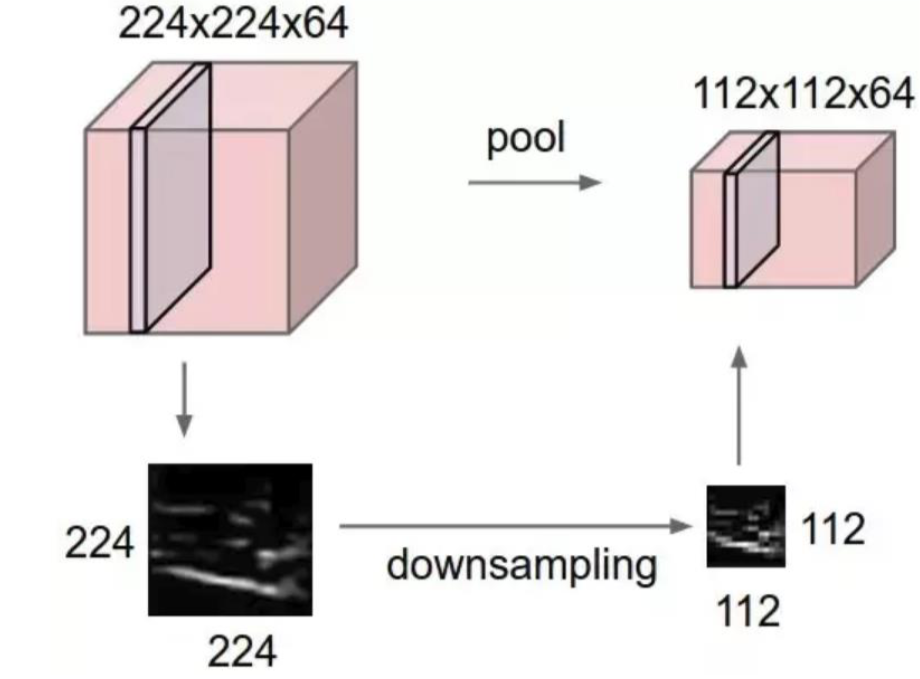
\includegraphics[width=1\textwidth]{Machine Learning in Computer Visualisation/img/MaxPooling2.PNG}
         \caption{Max pooling in a newtwork}
     \end{subfigure}
\end{figure}

\begin{center}
	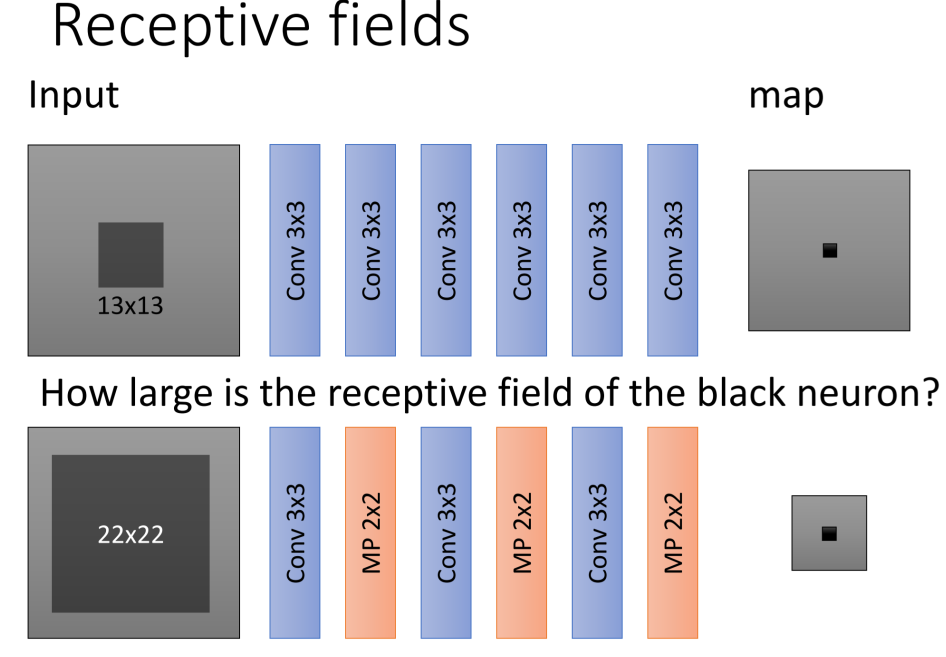
\includegraphics[width=0.5\linewidth]{Machine Learning in Computer Visualisation/img/MaxPooling3.PNG}
\end{center}

\subsubsection{Typical architecture}
\begin{figure}[H]
     \centering
     \begin{subfigure}[b]{0.45\textwidth}
         \centering
         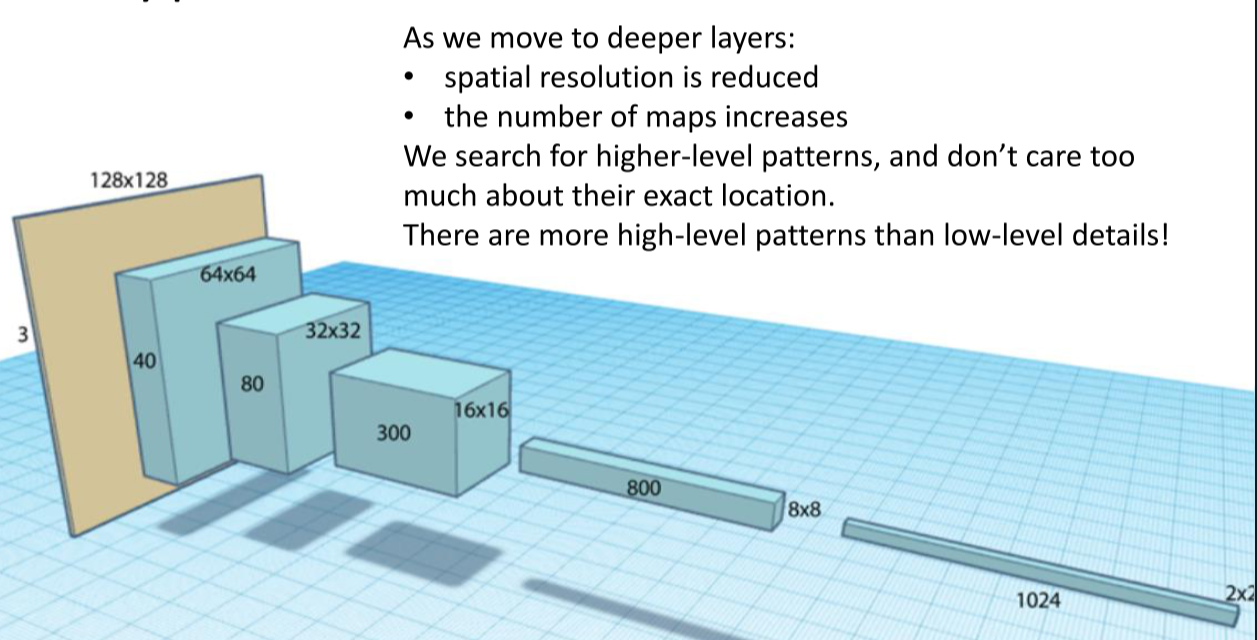
\includegraphics[width=0.95\textwidth]{Machine Learning in Computer Visualisation/img/typArch1.PNG}
         \caption{Typical architecture}
     \end{subfigure}
     \hfill
     \begin{subfigure}[b]{0.45\textwidth}
         \centering
         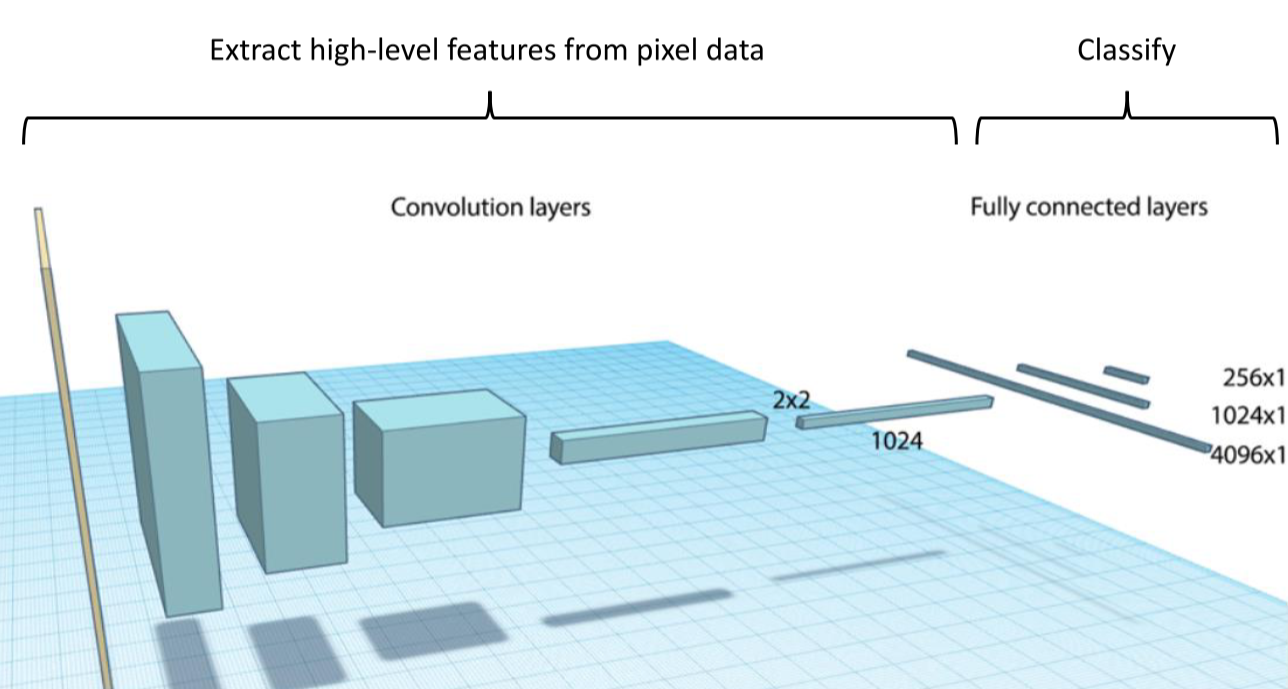
\includegraphics[width=1\textwidth]{Machine Learning in Computer Visualisation/img/typArch2.PNG}
         \caption{Typical architecture}
     \end{subfigure}
\end{figure}

\subsubsection{Software stack}
\begin{center}
	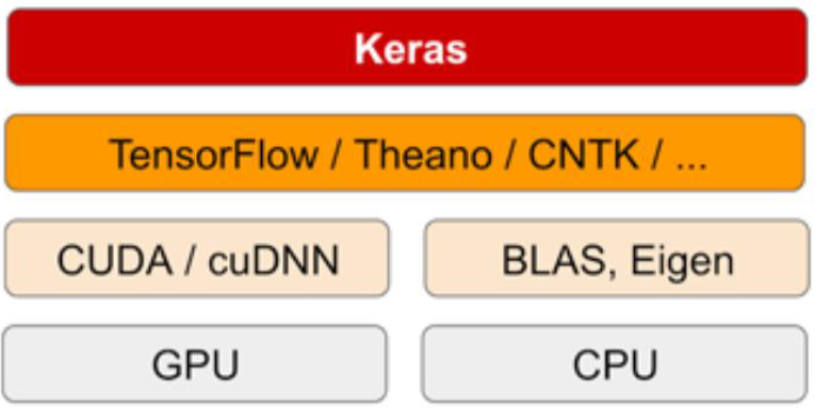
\includegraphics[width=0.5\linewidth]{Machine Learning in Computer Visualisation/img/softwareStack.PNG}
\end{center}

\section{Semantic Segmentation}
Identify pixels in images belonging to a specific class, sometimes additionally identifying pixels to belong to a specific instance of a class. It can thus be understood as supervised learning at the pixel level.
\begin{center}
	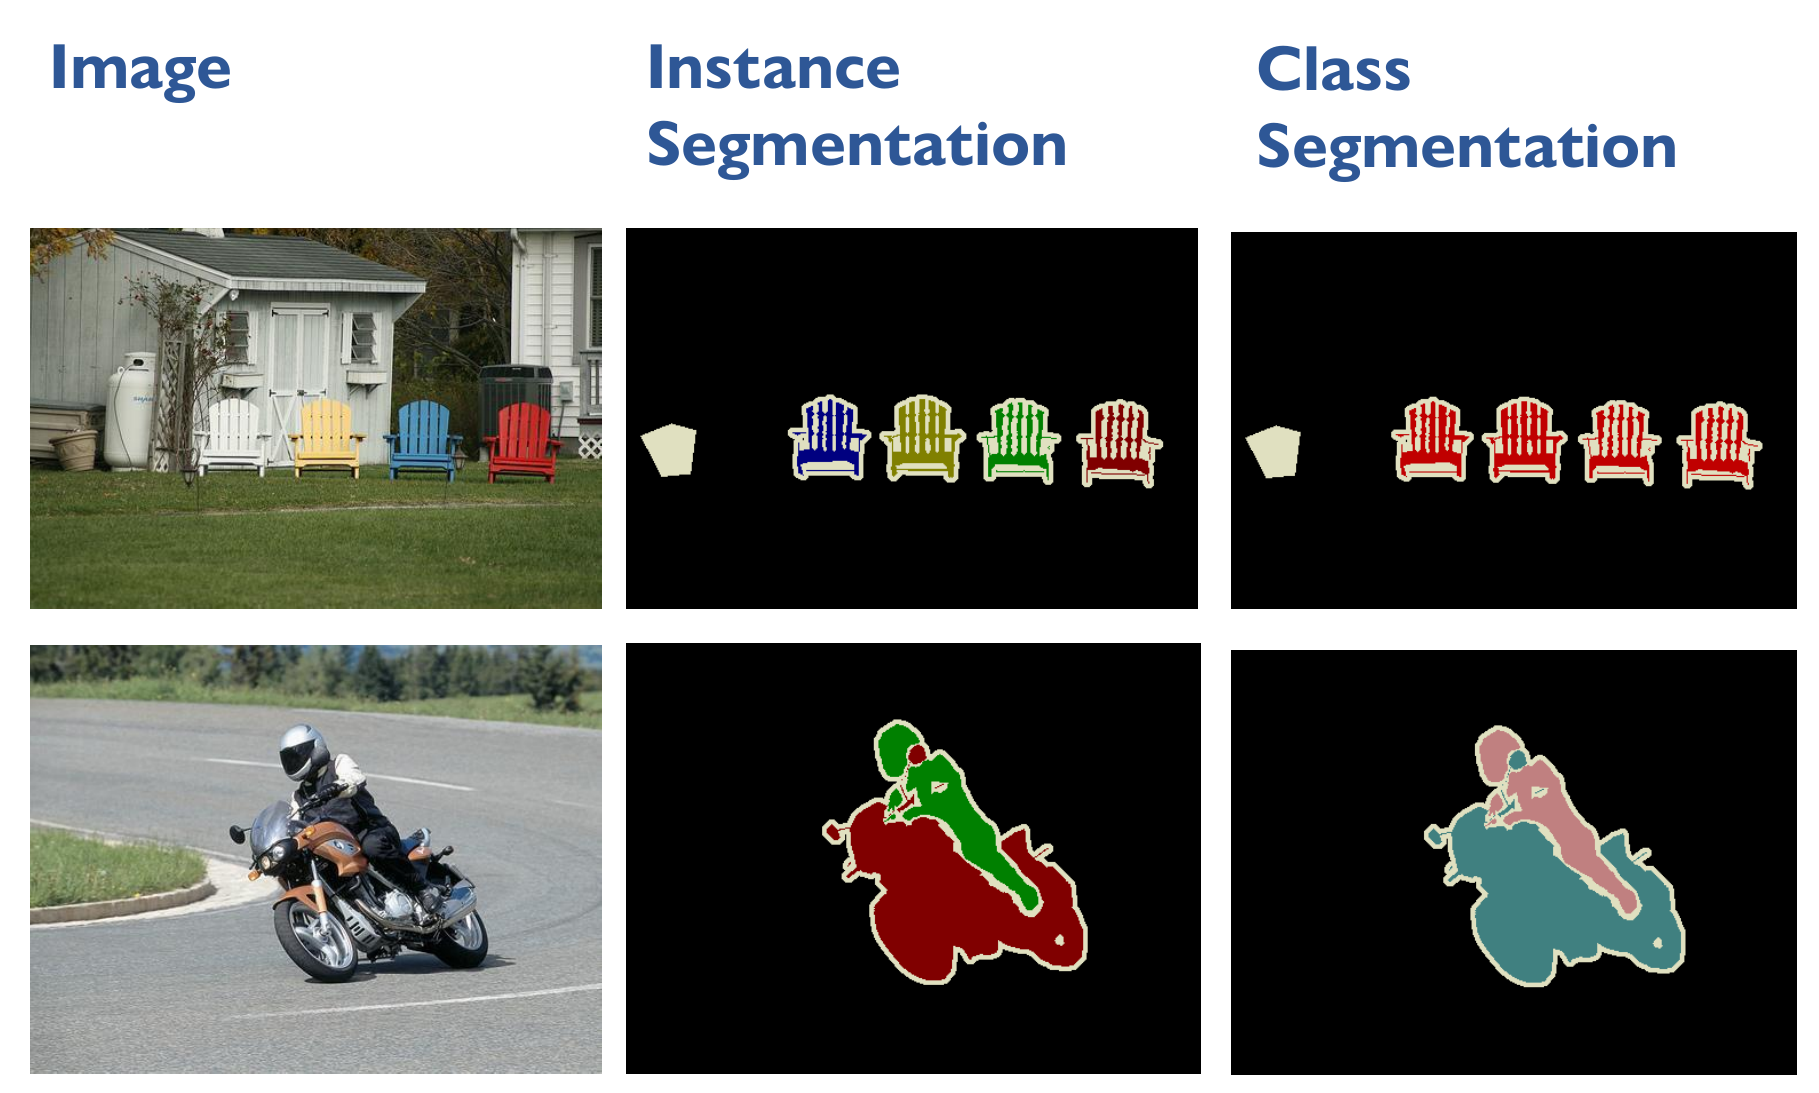
\includegraphics[width=0.7\linewidth]{Machine Learning in Computer Visualisation/img/semantic_segmentation.png}
\end{center}
Non-semantic segmentation tries to find regions in images without any additional information like classes or similar. It is thus similar to unsupervised learning and often a bottom-up approach. Segmentation in general tries to find a compact representation of a scene in terms of regions which share common properties.
\subsection{Overview}
\begin{center}
	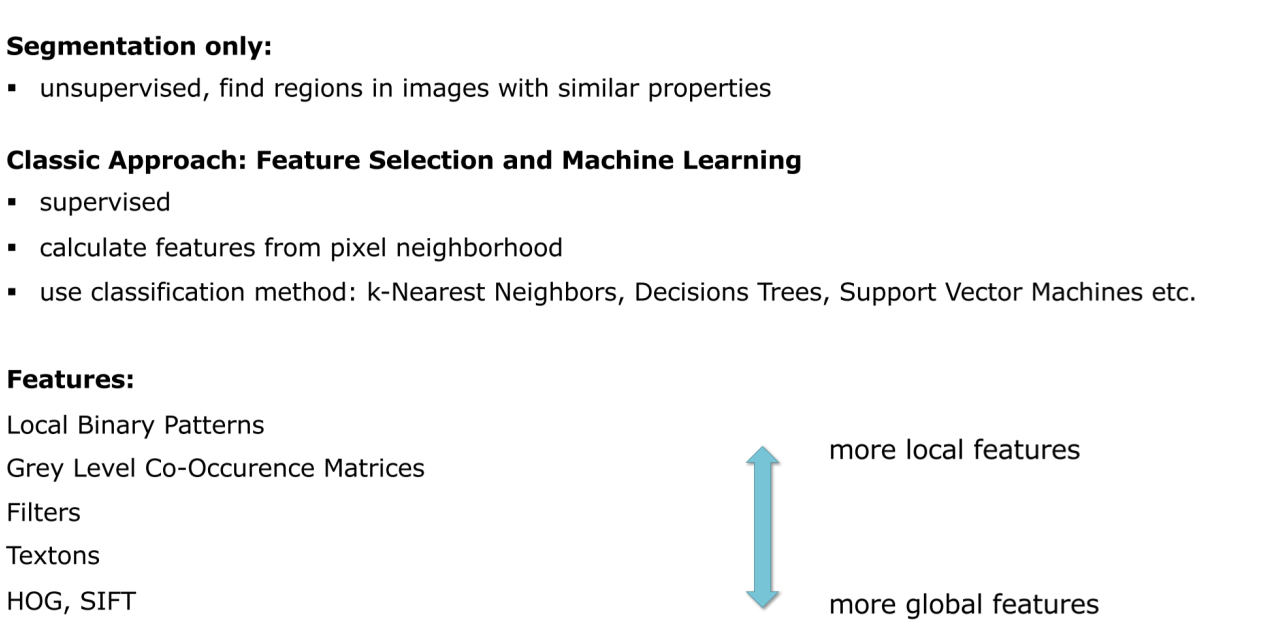
\includegraphics[width=1\linewidth]{Machine Learning in Computer Visualisation/img/semseguebersicht.PNG}
\end{center}


\subsection{Split and Merge AND Watershed}
Watershed and Split and Merge are both supervised learning approaches. \newline
\textbf{Split and Merge}
\begin{enumerate}
    \item Split inhomogeneous regions in the image recursively (Split)
    \item Merge neighboring regions with matching properties (Merge)
\end{enumerate}

\textbf{Watershed}
\begin{itemize}
    \item Interpret the image as a height map
    \item Fill the image with water
    \item Calculate lines of watersheds
\end{itemize}

\begin{figure}[H]
     \centering
     \begin{subfigure}[b]{0.45\textwidth}
         \centering
         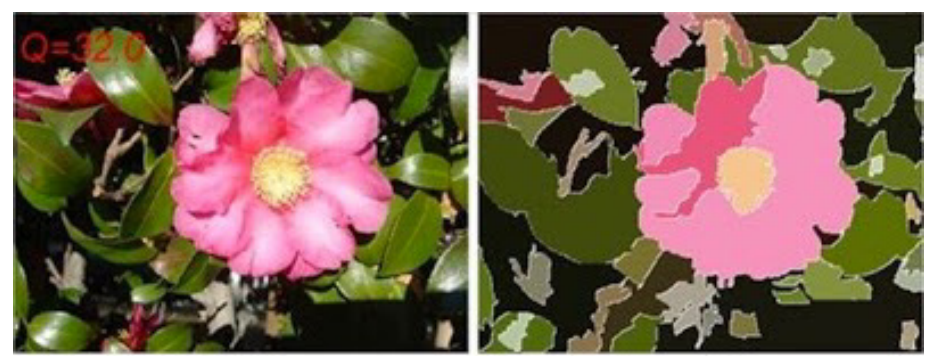
\includegraphics[width=0.95\textwidth]{Machine Learning in Computer Visualisation/img/splittAndMerge.PNG}
         \caption{Split and Merge}
     \end{subfigure}
     \hfill
     \begin{subfigure}[b]{0.45\textwidth}
         \centering
         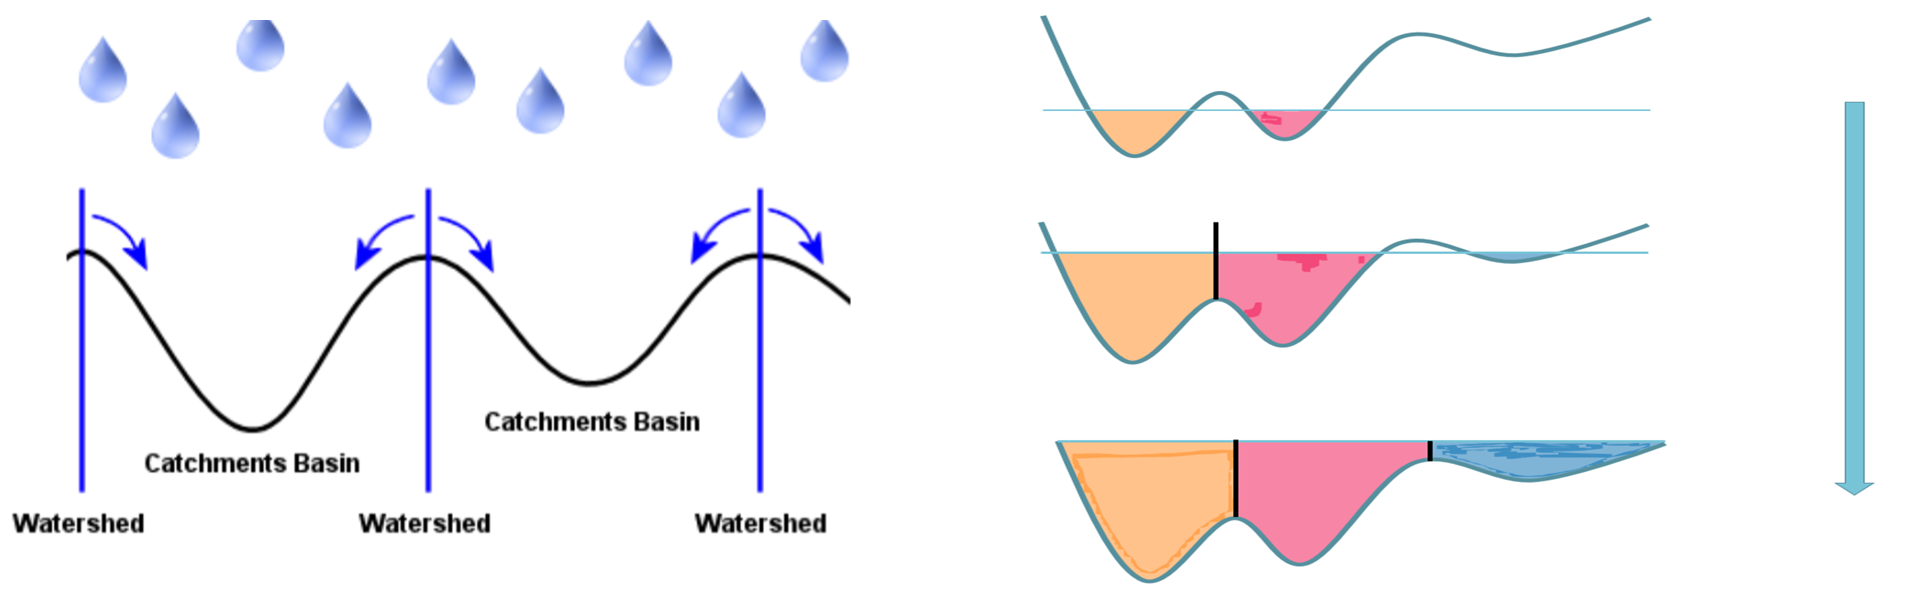
\includegraphics[width=1\textwidth]{Machine Learning in Computer Visualisation/img/Watershed.png}
         \caption{Watershed}
     \end{subfigure}
\end{figure}

+\subsection{k-Means Clustering}
Is not an optimal solution to cluster an image. Lloyds algorithm is one possibility to do clustering
\begin{enumerate}
	\item[-\ ] Initialise cluster centers (for example randomly)
	\item Calculate which samples belong to which clusters
	\item Calculate mean values of clusters as new centres
	\item[-\ ] Iterate until clusters don't change
\end{enumerate}


\begin{figure}[H]
     \centering
     \begin{subfigure}[b]{0.45\textwidth}
        \textbf{Problems:}
        \begin{itemize}
	    \item Number of clusters must be given
	    \item Cluster shapes are given (spherical)
        \end{itemize}
     \end{subfigure}
     \hfill
     \begin{subfigure}[b]{0.45\textwidth}
        \textbf{What can be clustered:}
        \begin{itemize}
	    \item Anything e.g.
         \item RGB values
         \item HSV values
         \item Position
         \item Color and position
        \end{itemize}
     \end{subfigure}
\end{figure}



\subsection{Mean Shift Clustering}
The shape of the clusters should be variable and not be determined by the method. Mean shift clustering can be achieved by the algorithm
\begin{enumerate}
	\item Search for the maximum of the feature densitity from a given position in the image
	\item Define cluster as the set of positions that converge to the same maximum
\end{enumerate}
The problem to search for local maxima of the features without having a feature distribution available directly. The solution is to use a Kernel Density Estimation to describe the distribution, for example using the Gaussian kernel. Or using the Derivative of the Gaussian to get an approximation directly.
\begin{align*}
	\hat{f}_h(x) &= \frac{1}{nh}\sum_{i=1}^{n}K\left(\frac{x-x_i}{h}\right)\\
	K\left(\frac{x-x_i}{h}\right) &= \frac{1}{\sqrt{2\pi}} e^{-\frac{(x-x_i)^2}{2h^2}}
\end{align*}
\begin{center}
	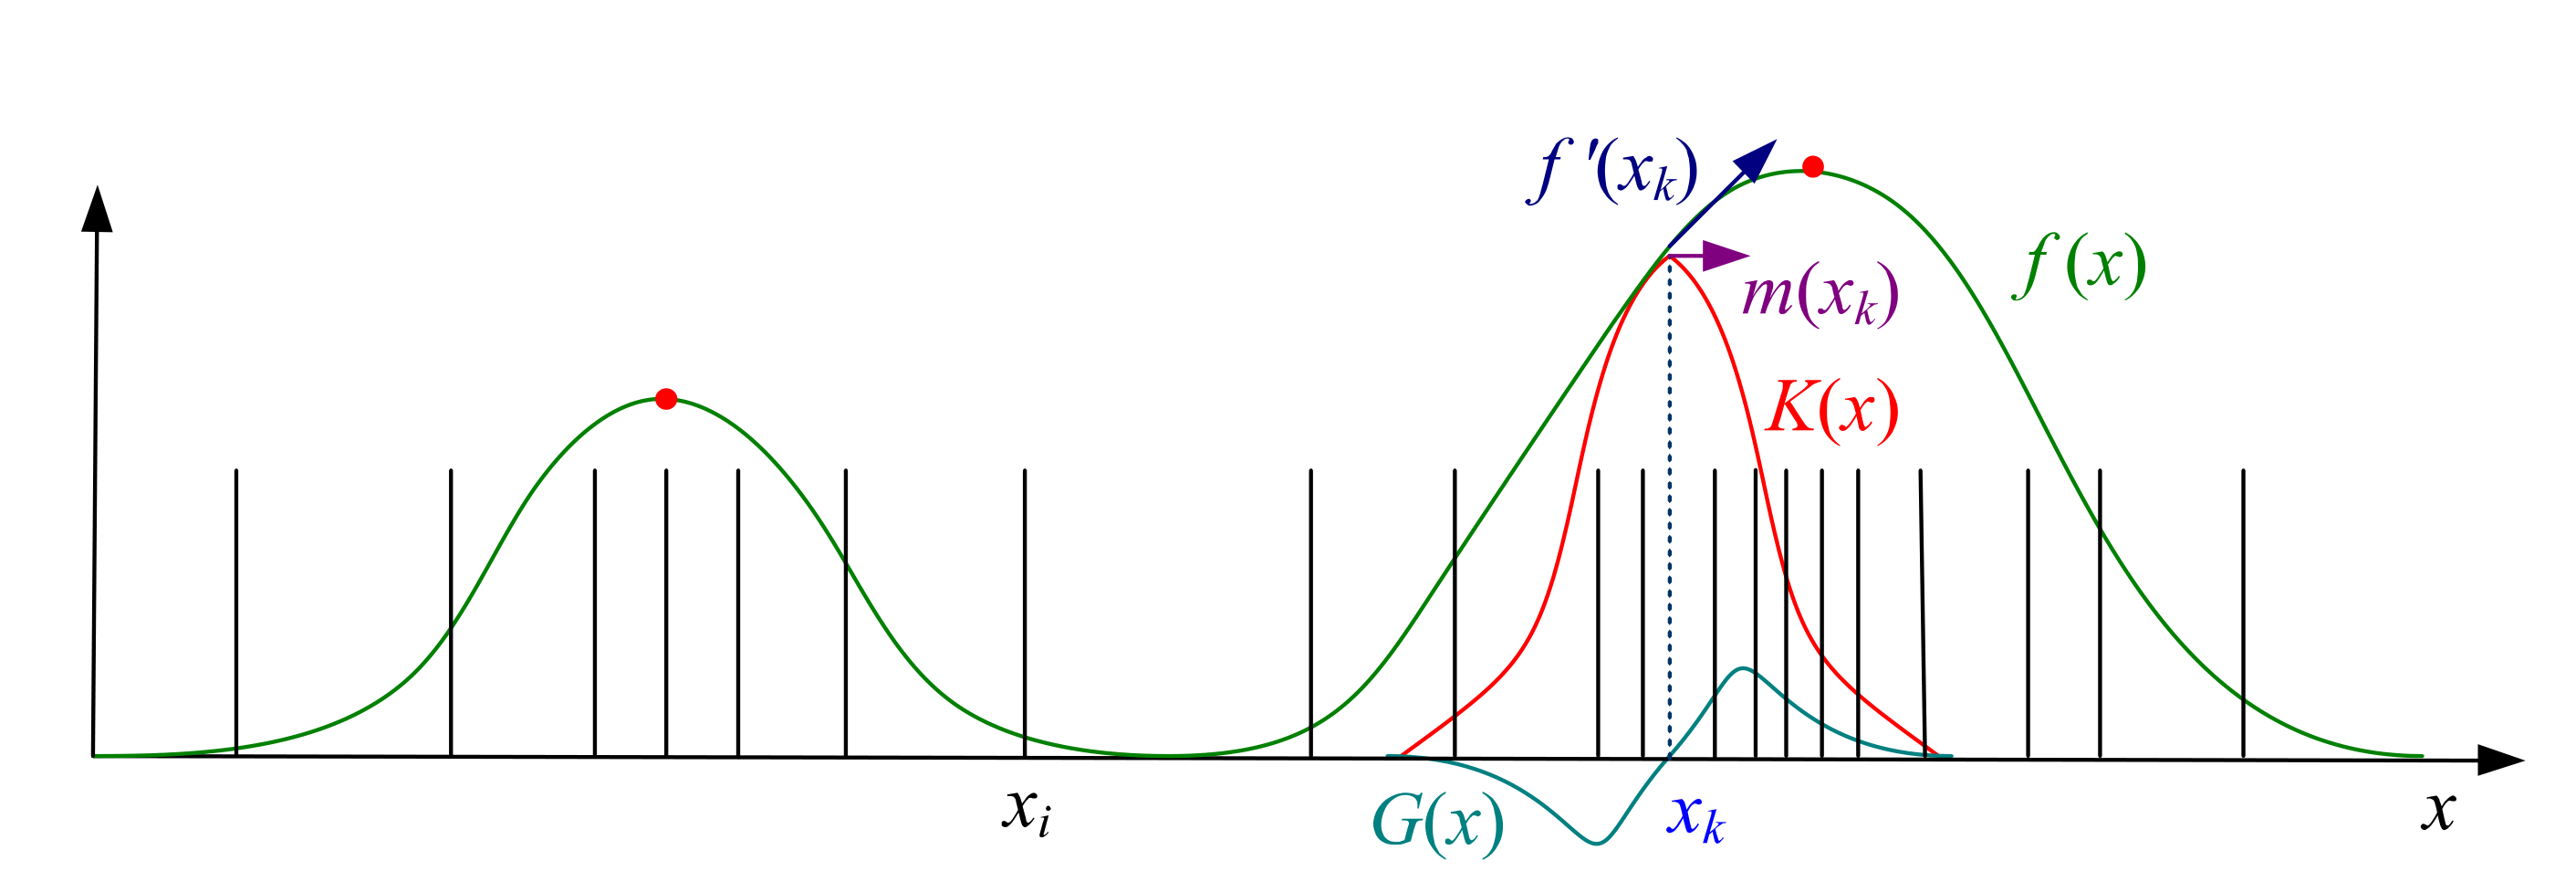
\includegraphics[width=0.7\linewidth]{Machine Learning in Computer Visualisation/img/kernel_density_estimation.png}
\end{center}

\subsubsection{Mean Shift Algorithm}
\begin{itemize}[label=-]
	\item[] For all positions $x$ in the image
	\item Calculate the mean $m(x)$ in the environment $N(x)$
	\begin{equation*}
		m(x) = \frac{\sum_{x_i \in N(x)} K(x_i - x) x_i }{\sum_{x_i \in N(x)} K(x_i - x)}
	\end{equation*}
	\item Set $x$ to the mean $m(x)$
	\item Iterate until $x$ does not change
\end{itemize}
\textbf{Attraction basins} are regions from which all trajectories lead to the same node.

\begin{figure}[H]
     \centering
     \begin{subfigure}[b]{0.45\textwidth}
         \centering
         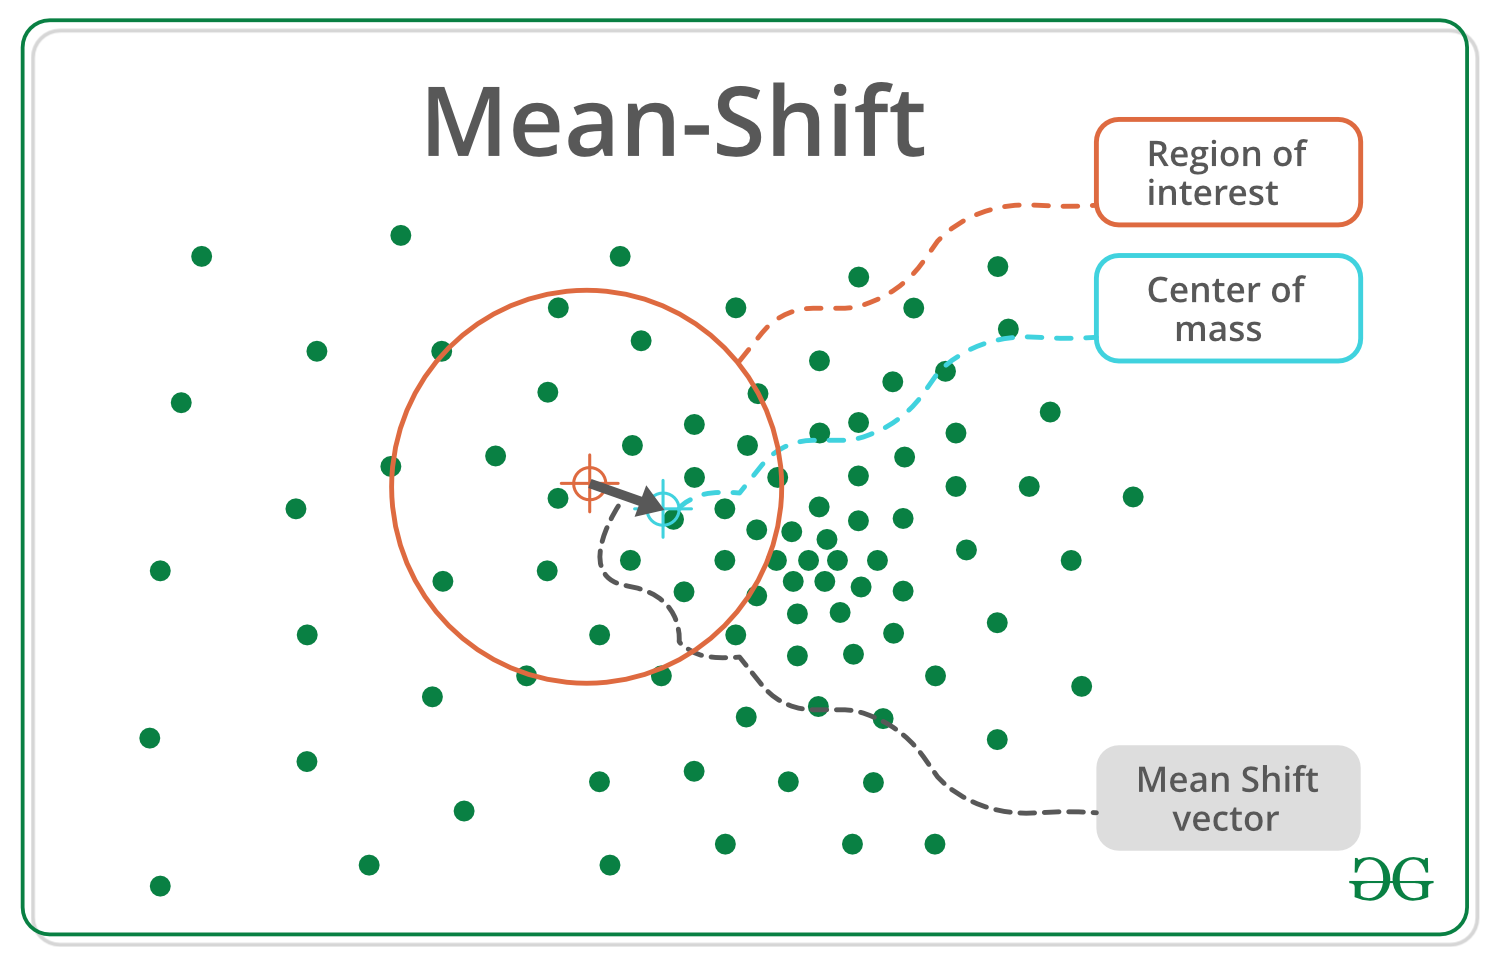
\includegraphics[width=0.95\textwidth]{Machine Learning in Computer Visualisation/img/Meanshift.png}
         \caption{Meanshift with attraction vector}
     \end{subfigure}
     \hfill
     \begin{subfigure}[b]{0.45\textwidth}
         \centering
         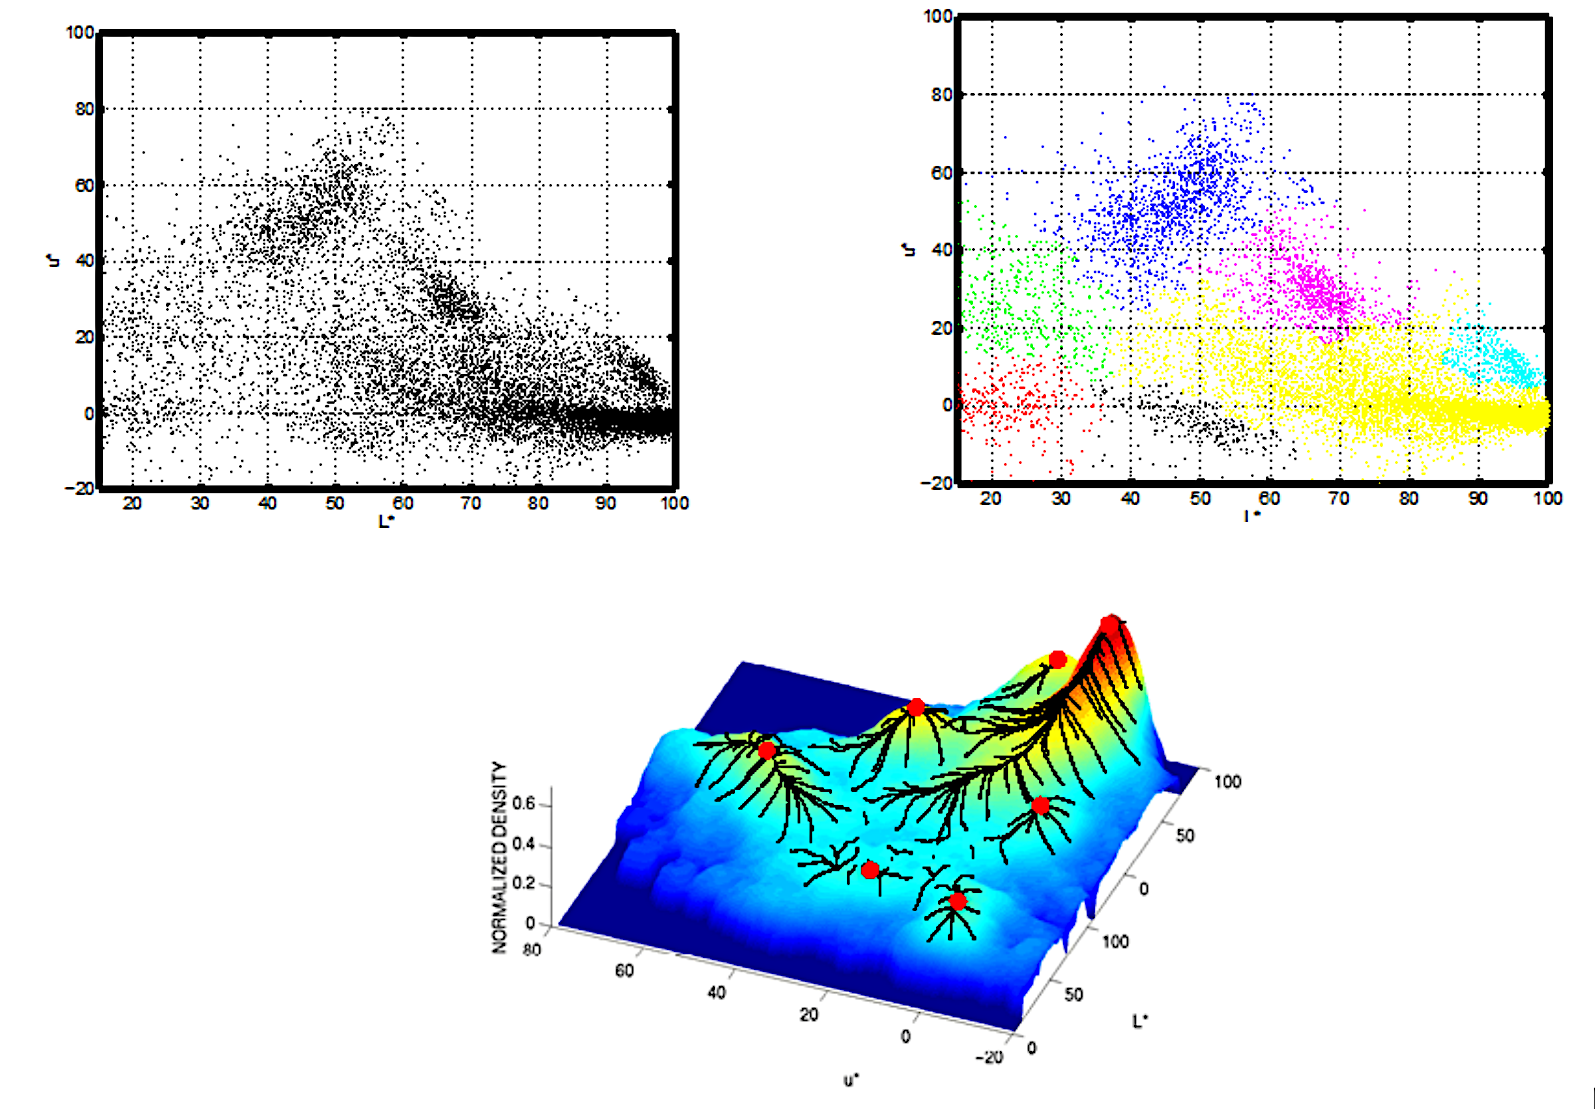
\includegraphics[width=1\linewidth]{Machine Learning in Computer Visualisation/img/attraction_basins.png}
         \caption{3D}
     \end{subfigure}
\end{figure}



\subsection{Segmentation by Graph Cuts}
Images are seen as graph with a node for every pixel with edges between nodes with an affinity weight for each edge. This weight  measures similarity, for example inversely proportional to difference in colour and position.
\begin{definition}
	Let $G=(V,E)$ be a graph. Each edge $(u,v)$ has a weight $w(u,v)$ that represents the similarity between $u$ and $v$. Cut $G$ into two disjoint graphs with node sets $A$ and $B$ by removing all edges between those sets. Assign a value to the cut as follows
	\begin{equation*}
		\text{cut}(A,B) = \sum_{u\in A,v\in B}^{w(u,v)}
	\end{equation*}
\end{definition}
Minimal value cuts often cuts too small groups. A better approach is to use normalised cuts:
\begin{align*}
	\text{Ncut}(A,B) &= \frac{\text{cut}(A,B)}{\text{assoc}(A,V)} + \frac{\text{cut}(A,B)}{\text{assoc}(B,V)}\\
	\text{assoc}(A,V) &= \sum_{u\in A, t\in V}^{w(u,t)}
\end{align*}
where $V$ is the set of all vertices.

\begin{figure}[H]
     \centering
     \begin{subfigure}[b]{0.45\textwidth}
         \centering
         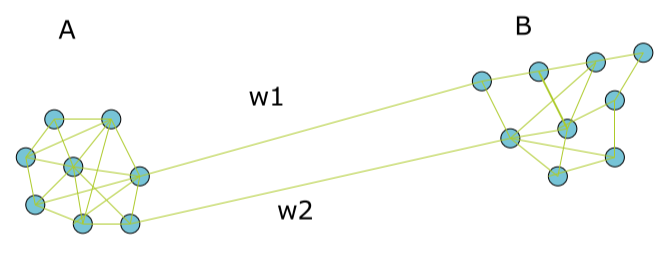
\includegraphics[width=0.95\textwidth]{Machine Learning in Computer Visualisation/img/GraphCut1.PNG}
         \caption{Definition}
     \end{subfigure}
     \hfill
     \begin{subfigure}[b]{0.45\textwidth}
         \centering
         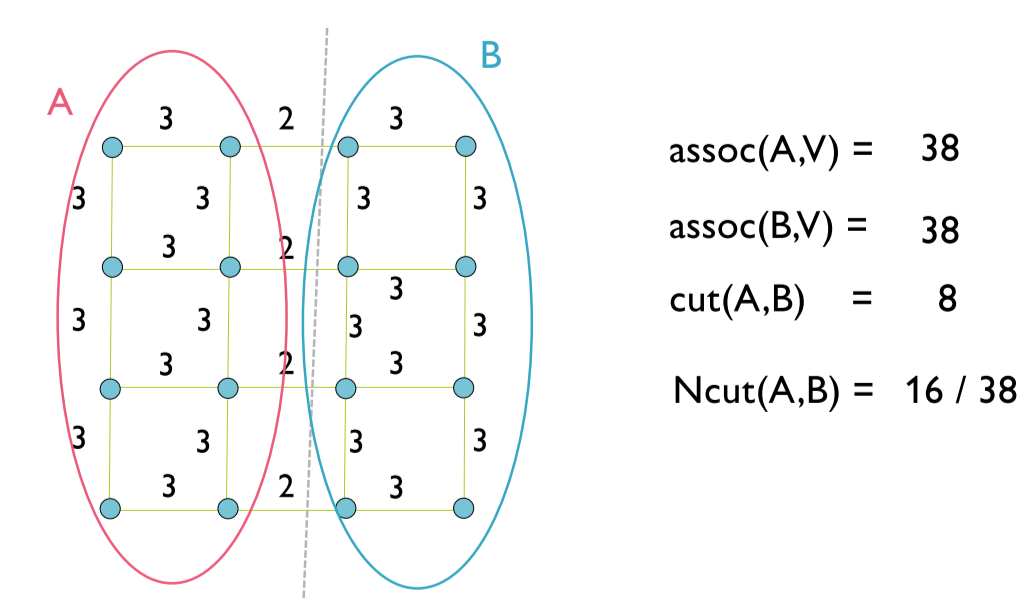
\includegraphics[width=1\linewidth]{Machine Learning in Computer Visualisation/img/GraphCut2.PNG}
         \caption{Calculated cut}
     \end{subfigure}
\end{figure}


\subsection{Superpixels}
The problem is that images contain many pixels and it is thus inefficient for graph calculations. The solution is to calculate \emph{superpixels} by grouping similar pixels first. This is cheap but leads to over-segmentation. As soon as the superpixels are calculated, normalised graph cuts can be applied.
\begin{center}
	\includegraphics[width=0.5\linewidth]{Machine Learning in Computer Visualisation/img/superpixels.PNG}
\end{center}

\subsubsection{Simple linear iterative clustering (SLIC)}
Simple linear iterative clustering is a fast method to calculate superpixels.
\begin{itemize}
    \item Superpixels are regions with no internal edges
    \item The number of approximate superpixels is given
    \item Cluster centers are initialized regularly
    \item Local clusters are found in the space (L a b x y) i.e. color and position
\end{itemize}

\subsection{K- Nearest Neighboar}
Supervised classification.\newline
Use the label of the k nearest neighbors.
\begin{figure}[H]
     \centering
     \begin{subfigure}[b]{0.45\textwidth}
         \centering
         \includegraphics[width=0.95\textwidth]{Machine Learning in Computer Visualisation/img/kNear.PNG}
         \caption{Segment of k neighbors}
     \end{subfigure}
     \hfill
     \begin{subfigure}[b]{0.45\textwidth}
         \centering
         \includegraphics[width=1.2\linewidth]{Machine Learning in Computer Visualisation/img/linear.PNG}
         \caption{Linear function cut}
     \end{subfigure}
\end{figure}



\subsection{Support vector machine (SVM)}
Better than linear function.
\begin{itemize}
    \item Optimize: Margin as large as possible
    \item Minimize: penalty function for wrong samples
\end{itemize}

\begin{figure}[H]
     \centering
     \begin{subfigure}[b]{0.45\textwidth}
         \centering
         \includegraphics[width=1.2\textwidth]{Machine Learning in Computer Visualisation/img/SVM.PNG}
         \caption{Support vector machine}
     \end{subfigure}
     \hfill
     \begin{subfigure}[b]{0.45\textwidth}
         \centering
         \includegraphics[width=1\linewidth]{Machine Learning in Computer Visualisation/img/nonLinSVM.PNG}
         \caption{\textbf{Nonlinear SVM:} Transform inseparable data into a new space}
     \end{subfigure}
\end{figure}




\subsection{Features}
Usually, Raw Input pixel values are not used as input features, as this makes the input space too big. Instead a feature vector is calculated for each pixel or set of pixels. These feature calculate certain properties of an image or image region. Besides classification tasks, these vectors are also used to find subregion or image stitching, and more.

\subsubsection{Feature Properties}
Features should be invariant to
\begin{itemize}[label=-]
	\item Translation
	\item Rotation
	\item Scaling
	\item Illumination, colour changes
	\item Transformation (Skewing)
\end{itemize}

\subsubsection{Filter Banks}
\begin{center}
	\includegraphics[width=0.6\linewidth]{Machine Learning in Computer Visualisation/img/filter_bank.png}
\end{center}
\begin{itemize}
	\item RFS Filters: edge and line filters at six orientations and three scales, Gaussian and Laplacian of Gaussian
	\item MR8 Filters: Maxima of RFS Filters at each scale
\end{itemize}

\subsubsection{Texture Characteristics}
Textons use the texture descriptor as vectors of filter bank outputs. Textons found by clustering are called a dictionary generation. For comparison, use the similarity between regions in the Texton histograms directly.

\subsubsection{Grey Level Co-occurence Matrices (GLCMs)}
Measurement of how often a specific combination of a colour value between a pixel and its neighbours occur. This results in a $256\times 256$ matrix for the 256 grey values. Additional features like entropy, energy, homogeneity, contrast or dissimilarity can be calculated from the matrix.

\subsubsection{Scale Invariant Feature Transform (SIFT)}
Popular feature descriptor for various tasks such as object matching, image stitching and more. It is a combination of detector and descriptor. The descriptor uses the histogram of the gradient. SIFT results in a 128-dimensional vector.
\begin{center}
	\includegraphics[width=0.6\linewidth]{Machine Learning in Computer Visualisation/img/SIFT.png}
\end{center}

\subsubsection{Histogram of Oriented Gradients (HOG)}
Computes the gradient images in x and y, and divides the image into cells. Compute histogram of gradient orientation in cell, normalise and flatten it into a feature vector.

\subsubsection{HOGles}
"Invert" the HOG features to simulate the image that generates it. This is a helpful tool to understand bad detections.

\begin{figure}[H]
     \centering
     \begin{subfigure}[b]{0.45\textwidth}
         \centering
         \includegraphics[width=0.95\textwidth]{Machine Learning in Computer Visualisation/img/Hog.PNG}
         \caption{HOG}
     \end{subfigure}
     \hfill
     \begin{subfigure}[b]{0.45\textwidth}
         \centering
         \includegraphics[width=0.95\linewidth]{Machine Learning in Computer Visualisation/img/HOGles.png}
         \caption{Inverted HOG}
     \end{subfigure}
\end{figure}

\subsection{Metrics}
\begin{figure}[H]
     \centering
     \begin{subfigure}[b]{0.45\textwidth}
         \centering
         \begin{equation}
    Precision = \frac{tp}{tp+fp}
\end{equation}
\begin{equation}
    Recall = \frac{tp}{tp+fn}
\end{equation}
\begin{equation}
    Specificity = \frac{tn}{tn+fp}
\end{equation}
     \end{subfigure}
     \hfill
     \begin{subfigure}[b]{0.45\textwidth}
     \centering
    \begin{equation}
    Accuracy = \frac{tp+tn}{tp+tn+fp+fn}
\end{equation}
    \begin{equation}
    F1 = \frac{2tp}{2tp+fp+fn}
\end{equation}
    \begin{equation}
    IoU = \frac{tp}{tp+fp+fn}
\end{equation}
     \end{subfigure}
\end{figure}


\begin{figure}[H]
     \centering
     \begin{subfigure}[b]{0.45\textwidth}
         \centering
         \includegraphics[width=0.55\textwidth]{Machine Learning in Computer Visualisation/img/Metrics1.PNG}
         \caption{HOG}
     \end{subfigure}
     \hfill
     \begin{subfigure}[b]{0.45\textwidth}
         \centering
         \includegraphics[width=0.95\linewidth]{Machine Learning in Computer Visualisation/img/Metrics2.PNG}
         \caption{Inverted HOG}
     \end{subfigure}
\end{figure}


\section{CNN and Machine Learning in General}
Cnn networks.
\begin{center}
	\includegraphics[width=1\linewidth]{Machine Learning in Computer Visualisation/img/cnn.PNG}
\end{center}

\subsection{Up and Down sampling in neural networks}
\begin{center}
	\includegraphics[width=1\linewidth]{Machine Learning in Computer Visualisation/img/UpAndDownSamplingpng1.png}
\end{center}
\begin{center}
	\includegraphics[width=1\linewidth]{Machine Learning in Computer Visualisation/img/UpAndDownSamplingpng2.png}
\end{center}
\begin{center}
	\includegraphics[width=1\linewidth]{Machine Learning in Computer Visualisation/img/UpAndDownSamplingpng3.png}
\end{center}
\begin{center}
	\includegraphics[width=1\linewidth]{Machine Learning in Computer Visualisation/img/UpAndDownSamplingpng4.png}
\end{center}

This method is usually done with a U-Net or a SegNet architecture.
\begin{figure}[H]
     \centering
     \begin{subfigure}[b]{0.45\textwidth}
         \centering
         \includegraphics[width=0.95\textwidth]{Machine Learning in Computer Visualisation/img/UNET.PNG}
         \caption{U-Net}
     \end{subfigure}
     \hfill
     \begin{subfigure}[b]{0.45\textwidth}
         \centering
         \includegraphics[width=0.95\linewidth]{Machine Learning in Computer Visualisation/img/SegNet.PNG}
         \caption{SegNet}
     \end{subfigure}
\end{figure}

\subsection{Architectures}
\textbf{Residual network}
\begin{figure}[H]
     \centering
     \begin{subfigure}[b]{0.30\textwidth}
         \centering
         \includegraphics[width=0.95\textwidth]{Machine Learning in Computer Visualisation/img/residual1.PNG}
         \caption{U-Net}
     \end{subfigure}
     \hfill
     \begin{subfigure}[b]{0.69\textwidth}
         \centering
         \includegraphics[width=0.95\linewidth]{Machine Learning in Computer Visualisation/img/residual2.PNG}
         \caption{SegNet}
     \end{subfigure}
\end{figure}
\textbf{Vision Transformer}
\begin{center}
	\includegraphics[width=1\linewidth]{Machine Learning in Computer Visualisation/img/VisionTransormer.PNG}
\end{center}

\subsection{Deep neural networks}
Neural Networks: \textbf{Feature} $\rightarrow$ \textbf{Output} \newline
Deep Neural Networks: \textbf{Feature} $\rightarrow$ \textbf{Features} $\rightarrow$ \textbf{Output}
\subsubsection{Failures}
\begin{itemize}
    \item Overfitting
    \item Results too bad
    \item Uneven class distribution
    \item Does not learn anything
    \begin{itemize}
        \item different Model
        \item more parameters
    \end{itemize}
\end{itemize}

\subsubsection{Regularization}
Regularization means limiting the capacity.
\textbf{Capacity: }this is the number of parameters in the network.
Regularization methods:
\begin{itemize}
    \item $L^2$ Regularization $\Omega(\theta) = \frac{1}{2}\parallel w\parallel_{2}^2$ whereas $\parallel w\parallel_p = \sqrt[p]{W_1^p+W_2^p+...+W_n^p}$ 
    \item Use several models trained separately; vote for the best
    \item Dropout $\rightarrow$ Drop nodes; Set weights to 0
    \item Early stopping $\rightarrow$ Stop if error in validation increases again
\end{itemize}

\subsubsection{Batch Algorithm}
\begin{itemize}
    \item Used properties in optimization (for example the gradient) are expectations over the training set
    \item Calculating the expectations over the whole data set is very time consuming
    \item We can also calculate them by randomly sampling from the data set à Minibatch algorithms
\end{itemize}
\textbf{Minibatchsize "Hyperparameter"}
\begin{itemize}
    \item Larger batches $\rightarrow$ better estimates $\rightarrow$non-linear increasing costs
    \item Very small batch $\rightarrow$ underutilized hardware
    \item Memory might limit batch size
\end{itemize}
\textbf{Use adam or AdaGrade as optimizer}
\subsubsection{Batch Normalization and Activations functions}
Normalize the input from 0 to 1.
\textbf{Activation functions}
\begin{itemize}
    \item use ReLu
    \item Tryout Leaky Relu
    \item Possible try tanh; usually worse
    \item Don't use sigmoid in hidden layers
\end{itemize}
\begin{center}
	\includegraphics[width=1\linewidth]{Machine Learning in Computer Visualisation/img/actfunrtions.PNG}
\end{center}


\section{Finding Multiple Objects}
\begin{figure}[H]
     \centering
     \begin{subfigure}[b]{0.45\textwidth}
         \centering
         \textbf{Problems}
         \begin{itemize}
             \item Different backgrounds
             \item Illumination
             \item Occlusion (Fremdbestandteile)
             \item Deformation
             \item Interclass variants (Katzen rassen)
         \end{itemize}
     \end{subfigure}
     \hfill
     \begin{subfigure}[b]{0.45\textwidth}
         \centering
        \textbf{Algorithms}
        \begin{itemize}
            \item Classic
            \begin{itemize}
                \item Cascaded Classifier
                \item Viola Jones
                \item Face detector
            \end{itemize}
            \item Modern:
            \begin{itemize}
                \item RCNN
                \item YOLO
                \item SSD
            \end{itemize}
        \end{itemize}
     \end{subfigure}
\end{figure}


\subsection{Boosting}
Train weak classifiers and ad them up.
\begin{equation*}
	F(x) = \alpha_1 f_1(x) + \alpha_2 f_2(x) + \alpha_2 f_2(x) + \dots
\end{equation*}
Weak classifier used with $f$ feature, $\theta$ threshold and $p_j$ parity
\begin{equation*}
	h_j (\theta) = \left\{ \begin{matrix}
		1 & p_j f_j < p_j \theta_j\\
		0 & \text{otherwise}
		\end{matrix} \right.
\end{equation*}

\begin{center}
	\includegraphics[width=0.6\linewidth]{Machine Learning in Computer Visualisation/img/boosting.PNG}
\end{center}

\subsection{Intergral Image}
Fast calculation of filter results by using integrals images.
\begin{center}
	\includegraphics[width=1\linewidth]{Machine Learning in Computer Visualisation/img/intergral1.PNG}
\end{center}
\begin{center}
	\includegraphics[width=1\linewidth]{Machine Learning in Computer Visualisation/img/intergral2.PNG}
\end{center}

\subsection{Face Detection}
\begin{itemize}
    \item Use a sequence of individual classifiers
    \item Reject false result early
    \item Each step of the 10-step cascade is trained with Adaboost using 20 different features
\end{itemize}

\begin{center}
	\includegraphics[width=0.6\linewidth]{Machine Learning in Computer Visualisation/img/cascade_classifier_approach.png}
\end{center}

\subsection{Adaboost}
The first and second features selected by Adaboost.\newline
First feature $\rightarrow$ measures intensity between the eye region and the face
Second feature $\rightarrow$ compares the intensities in the eye region to the intensity across the bridges of the nose
\begin{center}
	\includegraphics[width=0.6\linewidth]{Machine Learning in Computer Visualisation/img/adaboost.PNG}
\end{center}

\subsection{Histogram of Oriented Gradients HOG for Human Detection}
Detection Pipeline
\begin{itemize}[label=-]
	\item Calculate HOG Descriptors
	\item Collect HOGs in Detection Window
	\item Use Linear SVM for Person or Non-Person Classification
\end{itemize}
\begin{center}
	\includegraphics[width=0.8\linewidth]{Machine Learning in Computer Visualisation/img/hog_human_detection.png}
\end{center}

\subsection{Region proposal by selective search}
\begin{center}
	\includegraphics[width=0.8\linewidth]{Machine Learning in Computer Visualisation/img/regionprob.PNG}
\end{center}

\subsection{OverFeat}
Combine Classification, Localisation and Detection.
\begin{itemize}[label=]
	\item Classification
	\begin{itemize}[label=-,nosep]
		\item CNN
		\item Sliding Windows, apply at every possible pixel and at multiple scales
		\item Subsampling factor of 12
	\end{itemize}
	\item Localisation
	\begin{itemize}[label=-,nosep]
		\item Generate Bounding Box Prediction, as a Regression Problem
		\item Uses the same first five layers in the CNN
	\end{itemize}
	\item Detection
	\begin{itemize}[label=-,nosep]
		\item Combine Classification and Localisation
		\item Merge and accumulate bounding boxes
	\end{itemize}
\end{itemize}

\begin{figure}[tbh]
	\centering
	\includegraphics[width=0.7\linewidth]{Machine Learning in Computer Visualisation/img/classification_localisation.png}
	\caption{Classification and Localisation visualised}
	\label{fig:classificationlocalisation}
\end{figure}

Sliding windows have the drawback of the huge numbers of different positions and sizes that need to be evaluated. A better idea would be to find image regions that are likely to contain an object, which are called region proposals.

\subsection{R-CNN}
Extract region proposals, compute CNN features on these, classify the regions using SVM.
\begin{center}
	\includegraphics[width=0.7\linewidth]{Machine Learning in Computer Visualisation/img/r-cnn.png}
\end{center}

\begin{center}
	\includegraphics[width=0.7\linewidth]{Machine Learning in Computer Visualisation/img/r-cnn_structure.png}
\end{center}

\subsubsection{Feature Extraction}
\begin{itemize}
	\item Proposal regions are warped to $227\times 227$ pixel images
	\item 4096 Features from $227\times 227$ RGB Image using five Convolutional and two fully connected layers from AlexNet Architecture
	\item Supervised pre-training on the ILSVRC2012 classification data set
	\item Domain-specific fine-tuning is done by continuing training on warped region proposals
\end{itemize}

\subsubsection{Classifier}
Use one linear SVM per class (one true class versus all others), consider regions with overlap of 30\% a positive example and treat the bounding box position as regression problem.

\subsubsection{FAST R-CNN}
Replace SVM of R-CNN with fully connected neural network for classification of objects and refined bounding boxes
\begin{center}
	\includegraphics[width=0.7\linewidth]{Machine Learning in Computer Visualisation/img/fast_r-cnn_structure.png}
	\includegraphics[width=0.7\linewidth]{Machine Learning in Computer Visualisation/img/fast_r-cnn_structure2.png}
\end{center}

\subsection{You Only Look Once (YOLO)}
YOLO is a Single Neural Network that predicts bounding boxes and classification probabilities, which is very Fast and has good classification but not so good localization properties. The approach is
\begin{itemize}[label=-,nosep]
	\item Divide Image into $S \times S$ grid
	\item Each grid cell predicts B bounding boxes with confidence scores ($x, z, w, h, \text{score}$)
	\item Each grid cell predicts class probabilities (independent of bounding boxes)
	\item Multiply confidence score and probabilities at test time
\end{itemize}

\begin{center}
	\includegraphics[width=0.7\linewidth]{Machine Learning in Computer Visualisation/img/yolo.PNG}
\end{center}

\subsubsection{Improvements}
\begin{itemize}[label=-]
	\item Add Batch Normalisation
	\item Use higher resolution ($448\times 448$)
	\item Use Anchor Bounding Boxes from k-Means Analysis on the training data
	\item Use new base net (darknet19 and darknet 58)
\end{itemize}

\subsubsection{Precision}
\textbf{Intersect of union}
Used for bounding boxes.\newline
False positive < Threshold < True positive
\begin{center}
	\includegraphics[width=0.7\linewidth]{Machine Learning in Computer Visualisation/img/intersectOfUnion.PNG}
\end{center}
\textbf{Mean average precision}
\begin{itemize}
    \item Mean average precision is the mean of the average precision (AP) of each class
    \item So calculate AP first for each class
    \item Then take the mean over all classes
\end{itemize}
\textbf{Average precision}
\begin{center}
	\includegraphics[width=1\linewidth]{Machine Learning in Computer Visualisation/img/Average precision.PNG}
\end{center}



\section{Generating Images}

\subsection{Conditional GANs for Image to Image Transfers}
A GAN learns the mapping from random noise $z$ to output image $y$
\begin{equation*}
	G: z \rightarrow y
\end{equation*}
A conditional GAN should learn the mapping from input image $x$ and noise $z$ to output image $y$
\begin{equation*}
	G: \{x,z\} \rightarrow y
\end{equation*}
In practice adding noise as input proves ineffective, as the network learns to ignore it. One solution is to use dropout as noise, both in training and during testing.
\begin{figure}[H]
	\centering
	\includegraphics[width=0.7\linewidth]{Machine Learning in Computer Visualisation/img/conditional_GAN_edge_map.png}
	\caption{In conditional GANs both the Generator $G$ and the Discriminator $D$ input the edge map}
	\label{fig:conditionalganedgemap}
\end{figure}

\subsubsection{Conditional GANs}
Generator Architectures
\begin{figure}[H]
	\centering
	\includegraphics[width=0.7\linewidth]{Machine Learning in Computer Visualisation/img/conditional_GAN_generator_architectures.png}
	\caption{U-Net architectures with connections between the layers seem to work better}
	\label{fig:conditionalgangeneratorarchitectures}
\end{figure}

\subsection{Neural Texture Synthesis}
Given a low resolution texture image can a larger image be generated? For this there are two main approaches
\begin{itemize}[label=-]
	\item Replicate pixels and patches using a suitable algorithm
	\item Find a model of the texture and generate new textures from the model
\end{itemize}

\subsubsection{Texture Synthesis Using CNNs}
Pass image$x$ through the network, the activations from each layer are then the feature maps $F^l \in \R^{N\times M}$ for the texture. Calculate the Gram matrix to compute correlations between feature maps (on the same layers)
\begin{equation*}
	G_{ij}^l = \sum_{k} F_{ik}^l F_{jk}^l
\end{equation*}
These Gram matrices describe the texture model.

\subsubsection{Generating Textures}
\begin{enumerate}[itemsep=0em]
	\item Start with noise image
	\item Use gradient descend to find another image that matches the Gram-matrix representation of the original image
	\item Optimize my minimizing the mean-squared distance between the matrices from the original and generated image
\end{enumerate}

\begin{center}
	\includegraphics[width=0.8\linewidth]{Machine Learning in Computer Visualisation/img/conditional_GAN_texture_generation.png}
\end{center}

\subsection{Neural Style Transfer}
\begin{center}
	\includegraphics[width=0.7\linewidth]{Machine Learning in Computer Visualisation/img/conditional_GAN_style_transfer.png}
\end{center}

\subsubsection{Content Representation}
Each input image generates filter responses $F^l \in \R^{N\times M}$ at each layer. Run gradient descend on noise images to find an image that generates the same response. If $F^l \in \R^{N\times M}$ is the response from the original image and $P^l \in \R^{N\times M}$ the response from the generated image, the loss is
\begin{equation*}
	\L_{\text{content}}(\vec{p},\vec{x},l) = \frac{1}{2} \sum_{i,j} (F_{ij}^l - P_{ij}^l)^2
\end{equation*}
Later layers in the network define the content

\subsubsection{Style Representation}
Each input image generates filter responses $F^l \in \R^{N\times M}$ at each layer, calculate Gram matrices from the features. If $A^l$ is the matrix from the original  image and $G^l$ the matrix from the generated image, the loss for one layer is
\begin{equation*}
	E_l = \frac{1}{4 N_l^2 M_l^2}\sum_{i,j}(G_{ij}^l - A_{ij}^l)^2
\end{equation*}
and including several layers
\begin{equation*}
	\L_{\text{style}}(\vec{a},\vec{x}) = \sum_{l=0}^{L}w_l E_l
\end{equation*}

\begin{center}
	\includegraphics[width=0.8\linewidth]{Machine Learning in Computer Visualisation/img/conditional_GAN_style_representation.png}
\end{center}

\subsubsection{Fast Style Transfer}
The problem is that style transfer is slow as it requires many passes through VNN, the solution is to train a neural network to perform style transfer. Train feedforward network for each style, use pretrained CNN with losses as before, and After training, stylize image with single forward pass.
\begin{center}
	\includegraphics[width=0.7\linewidth]{Machine Learning in Computer Visualisation/img/fast_style_transfer.png}
\end{center}

\clearpage
\appendix

\section{Python Code}
\subsection{Binarisation and Filtering}
\subsubsection{Binary Mask}
\begin{minted}{python}
mask = im > 0.8 # bright pixels will be True in the mask, others will be False 
plt.imshow(mask)
\end{minted}
\begin{center}
	\includegraphics[width=0.4\linewidth]{Machine Learning in Computer Visualisation/img/BinaryMask.png}
\end{center}

\subsubsection{Connected Component Analysis}
\begin{minted}{python}
import skimage.measure
labels = skimage.measure.label(im > 0.5)
print(labels.shape, labels.dtype)
print("Unique values in labels:", np.unique(labels))
> (303, 384) int64
> Unique values in labels: [  0   1   2   3   4   5   6   7   8   9  10
> 11  12  13  14  15  16  17  18  19  20  21  22  23  24  25  26  27  28
> 29  30  31  32  33  34  35  36  37  38  39  40  41  42  43  44  45  46
> 47  48  49  50  51  52  53  54  55  56  57  58  59  60  61  62  63  64
> 65  66  67  68  69  70  71  72  73  74  75  76  77  78  79  80  81  82
> 83  84  85  86  87  88  89  90  91  92  93  94  95  96  97  98  99 100
> 101 102 103 104 105 106 107  108 109 110 111 112 113 114 115 116 117 118 119]

regions = skimage.measure.regionprops(labels)

large_regions = [r for r in regions if r.area > 100]

# equivalent to
large_regions = []
for r in regions:
	if r.area > 100:
		large_regions.append(r)

print(f"There are {len(large_regions)} large regions")
> There are 25 large regions
\end{minted}
\noindent
The \mintinline{python}{regionprops} (documentation) function can compute properties for each connected component. Some important properties are the following:
\begin{itemize}[label=,nosep,leftmargin=*, labelindent=0.5cm]
	\item \mintinline{python}{area : int} Number of pixels of the region.
	\item \mintinline{python}{bbox : tuple} Bounding box (\texttt{min\_row, min\_col, max\_row, max\_col}). Pixels belonging to the bounding box are in the half-open interval \texttt{[min\_row; max\_row)} and [min\_col; max\_col).
	\item \mintinline{python}{centroid : array} Centroid coordinate tuple (row, col).
	\item \mintinline{python}{convex_area : int} Number of pixels of convex hull image, which is the smallest convex polygon that encloses the region.
	\item \mintinline{python}{label : int} The label in the labeled input image.
\end{itemize}

\begin{minted}{python}
import matplotlib.patches as patches
fig, ax = plt.subplots()
ax.imshow(im, cmap="gray")
for r in large_regions:
	(min_row, min_col, max_row, max_col) = r.bbox
	width = max_col - min_col
	height = max_row - min_row
	rect = patches.Rectangle((min_col,min_row),width,height,
	linewidth=1,edgecolor='b',facecolor='none')
	ax.add_patch(rect)
\end{minted}

\begin{minted}{python}
background = (np.min(im,axis=1,keepdims=True) * np.ones((1,im.shape[1])))

fig, axs = plt.subplots(ncols=2, nrows=2, figsize = (13,13))
axs[0,0].imshow(im, vmin=0, vmax=1)
axs[0,0].set(title="original")
axs[0,1].imshow(background, vmin=0, vmax=1)
axs[0,1].set(title="background")
axs[1,0].imshow(im - background, vmin=0, vmax=1)
axs[1,0].set(title="im - background")
mask = (im - background) > 0.25
axs[1,1].imshow(mask, vmin=0, vmax=1)
axs[1,1].set(title="binarized")
\end{minted}
\begin{center}
	\includegraphics[width=0.7\linewidth]{img/BinarizedRiceGrains}
\end{center}

\subsection{Model Fitting Hough Lines}
\begin{minted}{python}
import skimage.feature
import skimage.transform.hough_transform as ht
import matplotlib.pyplot as plt
import numpy as np

import skimage.data
import skimage.feature

im = skimage.data.camera()
imedges = skimage.feature.canny(im)

lines = ht.probabilistic_hough_line(imedges, threshold=100)
len(lines)

# Draw detected lines
fig,ax = plt.subplots(figsize=(10,10))

ax.imshow(im,cmap="gray")
for ((x0,y0),(x1,y1)) in lines:
ax.plot([x0,x1],[y0,y1],'b-')
\end{minted}

\subsection{Superpixel Segmentation}
\begin{minted}{python}
# import the necessary packages
from skimage.segmentation import slic
from skimage.segmentation import mark_boundaries
from skimage.util import img_as_float
from skimage import io
import matplotlib.pyplot as plt
import argparse

# construct the argument parser and parse the arguments
ap = argparse.ArgumentParser()
ap.add_argument("-i", "--image", required = True, help = "Path to the image")
args = vars(ap.parse_args())

# load the image and convert it to a floating point data type
image = img_as_float(io.imread(args["image"]))

# loop over the number of segments
for numSegments in (100, 200, 300):

# apply SLIC and extract (approximately) the supplied number
# of segments
segments = slic(image, n_segments = numSegments, sigma = 5)

# show the output of SLIC
fig = plt.figure("Superpixels -- %d segments" % (numSegments))
ax = fig.add_subplot(1, 1, 1)
ax.imshow(mark_boundaries(image, segments))
plt.axis("off")

# show the plots
plt.show()
\end{minted}
\end{document}
